%------------------------------------------------------------------------------
% Template file for the submission of papers to IUCr journals in LaTeX2e
% using the iucr document class
% Copyright 1999-2013 International Union of Crystallography
% Version 1.6 (28 March 2013)
%------------------------------------------------------------------------------

\documentclass{iucr}              % DO NOT DELETE THIS LINE
\usepackage{bm}
% \usepackage{graphicx}
% \usepackage{tabularx}
% \usepackage{subfigure}
% \usepackage{afterpage}
% \usepackage{sansmath}
\usepackage{mathtools}
% \usepackage{parskip}
% \usepackage{tikz}
% \usepackage{tikzorbital}
% \usepackage{setspace}
% \usepackage{xcolor}
% \usepackage{amssymb}
% \usepackage{bm}
\usepackage{amsmath}
% \usepackage{fancyhdr}
% \usepackage{rotating}
% \usepackage{siunitx}
\usepackage[hyphens,spaces,obeyspaces]{url}
\usepackage{color}

\newcommand{\todo}[1]{{\color{red}[TODO: "#1'']}}
\newcommand{\manuel}[1]{{\color{red}[Manuel: #1]}}
\newcommand{\inblue}[1]{{\color{blue}#1}}
\newcommand{\inred}[1]{{\color{red}#1}}
\newcommand{\ingreen}[1]{{\color{green}#1}}


     %-------------------------------------------------------------------------
     % Infobrmation about journal to which submitted
     %-------------------------------------------------------------------------
     \journalcode{S}              % Indicate the journal to which submitted
                                  %   A - Acta Crystallographica Section A
                                  %   B - Acta Crystallographica Section B
                                  %   C - Acta Crystallographica Section C
                                  %   D - Acta Crystallographica Section D
                                  %   E - Acta Crystallographica Section E
                                  %   F - Acta Crystallographica Section F
                                  %   J - Journal of Applied Crystallography
                                  %   M - IUCrJ
                                  %   S - Journal of Synchrotron Radiation

\begin{document}                  % DO NOT DELETE THIS LINE

     %-------------------------------------------------------------------------
     % The introductory (header) part of the paper
     %-------------------------------------------------------------------------

     % The title of the paper. Use \shorttitle to indicate an abbreviated title
     % for use in running heads (you will need to uncomment it).

\title{Free-space wavefront propagators for synchrotron radiation}
% * <msanchezdelrio@gmail.com> 2018-09-25T09:38:50.716Z:
%
% ^.
%\shorttitle{Short Title}

     % Authors' names and addresses. Use \cauthor for the main (contact) author.
     % Use \author for all other authors. Use \aff for authors' affiliations.
     % Use lower-case letters in square brackets to link authors to their
     % affiliations; if there is only one affiliation address, remove the [a].

\cauthor[a]{Manuel}{Sanchez del Rio}{srio@esrf.eu}{address if different from \aff}
\author[b]{Sajid}{ Ali}
\author[a]{Rafael}{Celestre}
\author[c]{Oleg}{Chubar}
\author[a]{Vincent}{Favre-Nicolin}
\author[a]{Jean-Pierre}{Guigay}
\author[d,b]{Chris}{Jacobsen}
\author[e]{David M.}{Paganin}
\author[a]{Giovanni}{Pirro}
\author[d]{Luca}{Rebuffi}



\aff[a]{European Synchrotron Radiation Facility, 71 Avenue des Martyrs F-38000 Grenoble \country{France}}
\aff[b]{Department of Physics \& Astronomy, Northwestern University, 2145 Sheridan Road, Evanston, Illinois 60208, \country{USA}}
\aff[c]{Brookhaven National Laboratory, 740 Ring Road, 11973 Upton, New York, \country{USA}}
\aff[d]{Argonne National Laboratory, 9700 South Cass Avenue, Lemont, Illinois 60439, \country{USA}}
\aff[e]{School of Physics and Astronomy, Monash University, \city{Victoria} 3800, \country{Australia}}

     % Use \shortauthor to indicate an abbreviated author list for use in
     % running heads (you will need to uncomment it).

%\shortauthor{Soape, Author and Doe}

     % Use \vita if required to give biographical details (for authors of
     % invited review papers only). Uncomment it.

%\vita{Author's biography}

     % Keywords (required for Journal of Synchrotron Radiation only)
     % Use the \keyword macro for each word or phrase, e.g. 
     % \keyword{X-ray diffraction}\keyword{muscle}

%\keyword{keyword}

     % PDB and NDB reference codes for structures referenced in the article and
     % deposited with the Protein Data Bank and Nucleic Acids Database (Acta
     % Crystallographica Section D). Repeat for each separate structure e.g
     % \PDBref[dethiobiotin synthetase]{1byi} \NDBref[d(G$_4$CGC$_4$)]{ad0002}

%\PDBref[optional name]{refcode}
%\NDBref[optional name]{refcode}

\maketitle                        % DO NOT DELETE THIS LINE

\begin{synopsis}
Numerical implementation of the propagation of a wavefront in vacuum is fundamental for many synchrotron radiation applications related to modeling beamline optics and data analysis. Here the most commonly used methods and implementations are described. 
\end{synopsis}

\begin{abstract}
Abstract goes here.
\end{abstract}


     %-------------------------------------------------------------------------
     % The main body of the paper
     %-------------------------------------------------------------------------
     % Now enter the text of the document in multiple \section's, \subsection's
     % and \subsubsection's as required.

\section{Introduction}
\label{ch:intro}

The transport or propagation of the synchrotron beam in free space is of paramount importance in synchrotron radiation. 
The main role of a synchrotron beamline is to transport and condition the x-ray beam from the source to the sample. The beamlines are usually long, and many ``empty'' spaces interconnect optical elements (slits, mirrors, lenses, gratings, etc.). In an experiment, beams propagate through optics and the specimen itself before an intensity is recorded.  Thus the simulation of beam propagation is important for predicting the performance of synchrotron beamlines as well as various imaging experiments.

Beam propagation in vacuum may be considered as a first view as trivial and obvious. This may be the case in some applications the beam can be considered fully incoherent, so that ray-like geometrical size and divergence are sufficient to describe the transport. 
%X-rays are ``rays'' that travel in a straight line. 
However, improvements in x-ray sources mean that many beamlines and experiments utilize partially coherent beams. Here, X rays reveal wavelike behaviour and the synchrotron beam can be described by a wavefront or a collection of them. The transport of the wavefronts is governed by the wave equation. Because of the ``directional'' status of the synchrotron beam, it is important to know how to propagate a wavefield from a known value at $z=0$ to a downstream plane at a distance $z$.   Wave ``propagators'' are integral operators that act on the incident wavefront and permit to calculate the resulting transported wavefronts. Different propagators can be used depending on the characteristics of the system under study, in particular wavelength and propagation distance. 

For most applications, both in the domain of synchrotron instrumentation design (beamline optics) and for image reconstruction \cite{maiden_josaa_2012,gilles_optica_2018}, one has to use numeric calculations, thus implementing wave propagation in a computer code. A number of difficulties appear, related to the amount of data to be calculated, complexity of the equations, good sampling for optimizing computational time, and storage. Implementation methods, with their particularities and difficulties are described in different sections along the text. The simplest implementations rely on the discretization of the Fresnel propagator in one dimension and it is discussed in Section~\ref{ch: non-fourier-propagators}. This includes a description of artifacts that may appear in the results, replicas and aliasing. The section~\ref{ch: fourier-propagators} discusses the standard implementation of Fresnel propagators using Fourier transforms and show some basic examples of calculations that are compated with analytical results. This chapter also introduces a practical problem, the difficulty to sample correctly the phase when the wavefront is highly converging or diverging. Solutions are presented in Section~\ref{ch: spherical fronts} with some examples. In section~\ref{ch: discussion} some examples are studied and discussed.

Our goal is to present in a unified way the different methods for free space propagation employed in different software codes used for both beamline simulations and data analysis. We aim to describing rigorously some aspects of the propagation that are usually not detailed in code documentation and references. We will see that the right selection of the propagator and the validity conditions is essential for obtaining correct results, and we will give some recomendations for its use. Moreover, different codes do use different computational implementations, computer languages (C++, Python), hardware (CPUs, GPUs), and tools (parallel computers), each one optimized for different applications and user community. The discussion and examples presented try to give a wide (although incomplete) scenario of what is inside the software we use for simulating the propagation of the synchrotron light.   

\section{Theoretical background}
\label{ch: theory}

\todo{Chris Jacobsen comment: I would skip all of this and start by stating the Helmholtz Equation.  All of this is in standard textbooks. You can state that x-ray interactions are dominated by dielectric effects, leading to an x-ray index of refraction of $n=1-\delta-i\beta$.}

From Maxwell equations we derive in this section the vacuum wave equations that describes the spatial and temporal evolution of electromagnetic fields in free space. We introduce the approximation of scalar theory: the electromagnetic disturbance at a given point in space-time is described by a single complex number rather than by a electric (and/or magnetic) field vector. Once the time-dependent vacuum wave equation for scalar field is obtained, the field is described as a superposition of monochromatic waves, the spectral decomposition. Each monochromatic component of the decomposition of the electromagnetic field obeys the Helmholtz equation, a time-independent form of the free space wave equation. We will focus our attention on the study of diffraction of waves obeying the Helmholtz equation in free-space, and in particular on the case of Fresnel diffraction. All this arguments will be discussed based on a well-established approach \cite{paganin_book} using an angular spectrum formulation, thus representing the electromagnetic field as a superposition of monochromatic plane waves with different spatial frequency and direction of propagation. 

We start from Maxwell wave equations
\begin{equation}
\label{eq: Maxwell equations}
\begin{aligned}
\bm{\nabla} \times \bm{\mathcal{B}} &=\epsilon_0 \mu_0 \frac{\partial \bm{\mathcal{E}}}{\partial t}
&\qquad &\text{Faraday's law},\\[2\jot]
\bm{\nabla} \times \bm{\mathcal{E}} &= -\frac{\partial \bm{\mathcal{B}}}{\partial t}
&\qquad &\text{Amp\`{e}re's law},\\[2\jot]
\bm{\nabla} \cdot \bm{\mathcal{B}}    &= 0 & \qquad &\text{Gauss' law},\\[2\jot]
\bm{\nabla} \cdot \bm{\mathcal{E}}    &= 0 & \qquad &\text{Coulomb's law},
\end{aligned}
\end{equation}
where $\mathcal{B}$ is the magnetic induction, $\mathcal{E}$ is the electric field, $\mu_0$ and $\epsilon_0$ are the magnetic and the electric permittivity of free-space, respectively, $\nabla \times$ is the curl operator and $\nabla \cdot$ is the divergence operator. The vacuum wave equation that governs the spatial and temporal evolution of the electromagnetic field in free space will be derived. Note that $\mathcal{E}=\mathcal{E}(x,y,z,t)$ and $\mathcal{B}=\mathcal{B}(x,y,z,t)$ are functions of four variables. 

With some manipulations one can arrive to the wave equation for the electric field
\begin{equation}\label{eq: d'Alembert electric field}
	\Big(\epsilon_0 \mu_0 \frac{\partial^2}{\partial t^2}-\nabla^2\Big) \vec{\mathcal{E}} = \bm{0}.
\end{equation}
The same equation holds for the magnetic induction (replacing $\mathcal{E} \longleftrightarrow \mathcal{B}$). 
Note that since the vector Laplacian acts on the individual field components in the same way and keeping them uncoupled, the above vector equations, when projected onto $x$, $y$, or $z$ direction, split into 6 identical uncoupled equations, one for each field component.
This is known as the scalar wave equation of
\begin{equation}\label{eq: d'Alembert scalar field}
\Big(\frac{1}{c^2} \frac{\partial^2}{\partial t^2}-\nabla^2\Big) U(x,y,z,t) = 0,
\end{equation}
where the scalar $U(x,y,z,t)$ stands for any of the three component of the vector fields $\vec{\mathcal{E}}$ and $\vec{\mathcal{B}}$ and $c= 1/\sqrt{\mu_0 \epsilon_0}$ is the velocity of light in vacuum. This equations show that the electric and magnetic field that compose light are traveling wave fields. If we consider one propagation direction $z$, the electric field reduces to two components in direction perpendicular to $z$: $\mathcal{E}_\sigma(x,y,z=z_0,t)$ $\mathcal{E}_\pi(x,y,z=z_0,t)$. $\mathcal{E}_\sigma$ and $\mathcal{E}_\pi$ describe the two components of polarized light. If we ignore polarization, we can drop the vectorial description and consider $\mathcal{E}(x,y,z=z_0,t)$ as a scalar so the description of the electromagnetic field is now done with a scalar theory, which means that the electromagnetic disturbance is not described by two vectors, the electric field and the magnetic field, but by a single scalar field which is a function of position and time. Because the field functions are linear, solutions with different frequencies can be added to form wave-packet solutions. For this reason, fields with harmonic time dependence $e^{-i\omega t}$ are those studied in the following chapters. When substituting such field into equation \ref{eq: d'Alembert scalar field}, the result is
\begin{equation}\label{eq: Helmholtz equation}
	\big[\nabla^2 + k^2\big]U(x,y,z)=0.
\end{equation}
where $k= (2\pi)/\lambda$ is wavenumber corresponding to a wavelength $\lambda$, $\omega$ is the angular frequency of the radiation and $c=\lambda f$ the velocity of light in vacuum. This is the Helmholtz equation. The time dependence in $U$ can be factorized. In fact, the time solution for such equation is always the same while the spatial solution depends on the initial and boundary conditions. From here on, the time dependency of the field $U$ is not written. We then work with a complex scalar function that obeys the Helmholtz equation.

\subsection{The scalar theory of Diffraction}
\todo{complete and correct...}
It is not the scope of this paper to detail the rigorous theory of diffraction arising when solving the scalar Helmholtz equation for general boundary conditions. Its development is not trivial and need sophisticated mathematical tools, like the Green's theorem, with clever use of the boundary conditions. Refs.~\cite{bornwolf}, \cite{nieto} and other texts in Optics present this theory. The procedure is: 
\begin{itemize}
  \item Write the solution of Helmholz Equation in the form of the integral theorem of Helmholz and Kirchhoff. 
  \item Consider the Kirchhoff approximation, that assumes that the boundary values of the solution at the bondaries can be determined by geometrical optics.
  %\item Obtain the Rayleigh-Sommerfield diffraction integrals, two formulas corresponding to Dirichlet and Neumann boundary conditions, respectively. 
  \item Obtain the Fresnel-Kirchhoff diffraction formula
  \item deduce the Fresnel diffraction formula
\end{itemize}
% 
The results of this scenario are the more intuitive approach called the angular spectrum method that is presented in the next section. It has the advantage of being more intuitive and free from some of the subtle difficulties of boundary conditions encountered when solving the Helmholtz equation exploiting the Green's theorem while (cf. Goodman \cite{goodmanfourier}).


\subsection{Angular spectrum method}

Consider the case of a source that emits only in the half-space with a positive spatial coordinate $z$ that describes its position in a Cartesian system.
%The space is supposed to be free of electric charges and a monochromatic wave only is considered to propagate forward with respect to the z coordinate. 
The angular spectrum formalism permits to construct an operator which applied to the electric field of incident wave permits to calculate the propagated one over any plane parallel to the initial one downstream of the source. Starting with the previous Cartesian coordinate system $(x,y,z)$, where the axis $z$ in the positive direction is considered to be the optical axis, consider two parallel planes, $z=0$ and $z=\Delta z$ where $\Delta z$ is a positive value on the $z$-axis. Consider the space between the two planes to be in vacuum, which means that equation \ref{eq: Helmholtz equation} is here obeyed. The aim is to use such equation to get an explicit form of the operator that once applied to the forward propagating field $U(x,y,0)$ yields to the propagated wave-field $U(x,y,\Delta z)$ at the plane $z=\Delta z$. A simple example of propagation can be achieved with the special case of a plane wave forward propagating along the $z$-axis
\begin{equation} \label{eq: plane wave}
U^{(PW)}(x,y,z)=e^{i(k_xx+k_yy+k_zz)}
\end{equation}
These waves are solution of the Helmholtz equation provided that $k_x$,$k_y$,$k_z$ are respectively the three components of the wave-vector $\bm{k}$, with
\begin{equation}\label{eq: k definition}
k_x^2+k_y^2+k_z^2 =k^2 =\left( \frac{2 \pi}{\lambda} \right)^2.
\end{equation}
This vector gives the direction of propagation of the wave. Expressing $k_z$ as a function of $k$, $k_x$ and $k_y$ and taking the positive square root value which, as before, makes it so only propagation in the positive direction of the $z$-axis is considered:
\begin{equation} \label{eq: kz}
k_z = \sqrt{k^2 -k_x^2-k_y^2}
\end{equation}
By substituting equation \ref{eq: kz} into equation \ref{eq: plane wave}, one obtains
\begin{equation}\label{eq: plane wave with no kz}
U^{(PW)}(x,y,z)=e^{i(k_xx+k_yy)}e^{iz\sqrt{k^2 -k_x^2-k_y^2}}
\end{equation}
Now the plane wave at position $z=0$ is 
\begin{equation} \label{eq: plane wave with no kz at z=0}
U^{(PW)}(x,y,0)=e^{i(k_xx+k_yy)}.
\end{equation}
The trivial problem of diffraction for a plane wave has then been solved. In fact, to obtain the propagated wave field it simply a matter of multiplying the unpropagated disturbance by the propagation factor $e^{i z\sqrt{k^2 -k_x^2-k_y^2}}$, that will be called 'free space propagator'. Extending this result from a plane wave forward propagating in vacuum between two parallel planes at position $z=0$ and $z=\Delta z$ to a more general disturbance is a matter of expressing the general unpropagated wave field as a linear combination of plane waves through the use of two dimensional Fourier integral \todo{It would be nice to continue the discussion and arrive to the same results, if possible, without using the Fourier space. The discussion of Fourier-related aspects is in next section}
\begin{equation}\label{eq: Fourier transform of unpropagated field}
U(x, y, 0) = \frac {1}{ 2 \pi}\int \int \widetilde{U}(k_x, k_y, 0)e^{i(k_x x + k_y y)} dk_x dk_y
\end{equation} 
\todo{we use here a definition of FT different to the one in Appendix A}
where $\widetilde{U}(k_x, k_y, 0)$ denotes the Fourier transform of $U(x,y,0)$ with respect to $x$ and $y$ while $k_x$ and $k_y$ represent the spatial-frequencies coordinate in the Fourier space. By applying the propagator operator $e^{i z\sqrt{k^2 -k_x^2-k_y^2}}$ to the unpropagated field, as it was show before, it is possible to retrieve the value of the field $U(x,y,\Delta z)$ propagated by a distance $z=\Delta z$. In order to do so, it is necessary to multiply such propagator for every component in which the unpropagated field as been decomposed through the use of equation \ref{eq: Fourier transform of unpropagated field}, thus arriving at
\begin{equation}\label{eq: angular-spectrum representation}
U(x, y, \Delta z) = \frac {1}{ 2 \pi}\int \int \widetilde{U}(k_x, k_y, 0)e^{i\Delta z\sqrt{k^2 -k_x^2-k_y^2}}e^{i(k_x x + k_y y)} dk_x dk_y.
\end{equation} 
This is the \textbf{angular-spectrum representation} for propagated fields and it provides a rigorous solution to a certain boundary problem of the Helmholtz equation, namely one in which a forward propagation happens in free-space between two parallel planes. 

\subsection{Fresnel approximation}

We are interested to study the propagation of synchrotron radiation, a coherent X-ray beam that propagates making only small angles with respect to the $z$-axis. In this case the wave field is said to be 'paraxial'. In this special case, an approximation of the equation \ref{eq: angular-spectrum representation} leads to a simpler solution to the Helmholtz equation equivalent to the famous Fresnel diffraction integral. Starting from the previous general result, suppose that $U(x,y,0)$ is now a scalar function that describes a paraxial wave field. Since the paraxiality, as mentioned before, imply that all the non-negligible plane-wave components of the forward propagating field have small wavenumber components $k_x$ and $k_y$ such that $k_z << k_x, k_y$, it is possible to expand with Taylor expansion the square-root argument of the exponential of the free-space propagation:
\begin{equation}\label{eq: binomial approx}
\sqrt{k^2 -k_x^2-k_y^2}\approx k -\frac{k_x^2+k_y^2}{2k}	
\end{equation}
The propagated paraxial field is then described by a approximate form of the free-space propagator, called the \textbf{Fresnel propagator}
\begin{equation}\label{eq: Fresnel approx of angular spectrum}
U(x, y, \Delta z) = \frac {e^{i k \Delta z}}{ 2 \pi}\int \int \widetilde{U}(k_x, k_y)  e^{\frac{-i \Delta z (k_x^2 + k_y^2) }{2k}} e^{i(k_x x + k_y y)}dk_x dk_y.
\end{equation}
It is also interesting to write the propagated field $U(x,y,\Delta z)$ as a function of the incident field $U$ instead of its Fourier transform $\widetilde{U}$ as done in Eq.~\ref{eq: Fresnel approx of angular spectrum}. We will show in the next section but we anticipate here that this equation is equivalent to: 
\begin{equation}\label{eq: usualfresnel}
\boxed{
U(x,y, \Delta z) = \frac {e^{i k\Delta z }}{ i \lambda \Delta z} \int  \int U(x^\prime, y^\prime, 0) e^{i \frac{k}{2 \Delta z} [(x - x^\prime)^2 + (y - y^\prime)^2]} dx^\prime dy^\prime
}.
\end{equation}

This expression can be manipulated to extract some terms not depending on $x^\prime$ and $y^\prime$ outside of the integral
\begin{multline}\label{eq: fresnel2}
U(x,y, \Delta z) = \frac {e^{i k\Delta z }}{ i \lambda \Delta z}  e^{ i \frac{k}{2 \Delta z} (x^2 + y^2) } \times \\
\int \int \left\{ U(x^\prime, y^\prime, 0) e^{i \frac{k}{2 \Delta z} (x^{\prime 2} + y^{\prime 2} )} \right\} e^{-i \frac{k}{\Delta z} [x  x^\prime + y y^\prime]} dx^\prime dy^\prime .
\end{multline}

Equations~\ref{eq: usualfresnel} and \ref{eq: fresnel2} refer to the Fresnel propagator, and we recall it provides a rigorous solution of the Helmholtz equation for propagation in free space between two parallel planes using paraxial approximation. From the physical point of view, both equations are equivalent for propagation in the near and far field assuming paraxial approximation. However, for reasons that will be discussed in Section~\ref{ch: validity}, the numerical implementation would prefer Eq.~\ref{eq: usualfresnel} for near-field and Eq.~\ref{eq: fresnel2} for far field.

It is possible to demonstrate that the angular spectrum formalism developed here and the Rayleigh-Sommerfeld diffraction integral of the first kind yield identical predictions of diffracted fields. This was done elegantly by Sherman \cite{Sherman:67} and Lalor \cite{Lalor:68}. The text books of \cite{goodmanfourier}, \cite{nieto} and \cite{paganin_book} are examples where it is described the theoretical approach solving integral theorem of Helmholz and Kirchhoff to obtain the Fresnel-Kirchhoff and the Rayleigh-Sommerfeld diffraction formulas, depending on the choice of boundary conditions and Green functions. \todo{make clear the connection of the angular spectrum and other  theoretical formulations}

Synchrotron radiation is always well collimated along the propagation direction, therefore the use of the approximation \ref{eq: binomial approx} is justified in most cases. In the following we will assume this is true. For non-synchrotron applications, the calculation of the propagation of non-paraxial fields is sometimes needed. For that the use of higher orders of Taylor expansion may be needed, or other non-Taylor of expansions may be considered \cite{Mansuripur,Avoort}.


%
%%%%%%%%%%%%%%%%%%%%%%%%%%%%%%%%%%%%%%%%%%%%%%%%%%%%%%%%%%%%%%%%%%%%%%%%%%%%%%%%%%
%

\subsection{Far field (Fraunhofer) approximation}


The case when $e^{i \frac{k}{2 \Delta z} (x^{\prime 2} + y^{\prime 2} )} \simeq 1$ is called the Fraunhofer approximation, or far field approximation. From Eq.~\ref{eq: fresnel2} one obtains 
\begin{multline}\label{eq: fraunhoffer}
U(x,y, \Delta z) = \frac {e^{ik\Delta z }}{ i \lambda \Delta z}  e^{ i \frac{k}{2 \Delta z} (x^2 + y^2) } \times \\
\int \int  U(x^\prime, y^\prime, 0)  e^{-i \frac{k}{\Delta z} [x  x^\prime + y y^\prime]} dx^\prime dy^\prime .
\end{multline}
It is valid when the propagation distance verify $\Delta z >>k (x^{\prime 2}_{max} + y^{\prime 2}_{max})/2 $.  


\subsection{Fourier Optics}

The Fast Fourier Transform (FFT) algorithm (see, e.g., Ref.~\cite{10.2307/2003354}) is a clever implementation of the discrete Fourier transform in which the number of operations is greately reduced, from $\propto N^2$ that one obtain from the simple integral discretization to $\propto N \log_2 N$, where $N$ is the number of points of the array to be Fourier transform. The availability of performing libraries to compute FFT has revolutionized the numerical methods since its discovery in mid 60's. The importance is such that it helped to develop the ``Fourier Optics''. This has immediate application for calculating the propagator integral transforms. In this section we express the propagators obtained before in form of Fourier transforms. 

We recall that the convolution between two functions in 2D $f(x,y)$ and $g(x,y)$ is
\begin{equation}\label{eq: definition of convolution}
	f(x,y) * g(x,y) \coloneqq \int_{-\infty}^{\infty} \int_{-\infty}^{\infty} f(x^{\prime},y^{\prime})g(x-x^{\prime},y-y^{\prime})dx^{\prime}dy^{\prime}
\end{equation}
Using of the two-dimensional form of the convolution theorem (see, e.g., \cite{goodmanfourier}) of
\begin{equation}\label{eq: convolution theorem}
f(x,y) * g(x,y) = \mathcal{F}^{-1}\big\{{\mathcal{F}\{f(x,y)\} \times \mathcal{F}\{g(x,y)\}} \big\},
\end{equation}
one can write Equation \ref{eq: Fresnel approx of angular spectrum}  in a form that resemble a convolution in two dimensions:
\begin{align}\label{eq: convolution form of angular spectrum}
U(x, y, \Delta z) &= \mathcal{F}^{-1}\Big\{ \mathcal{F}\{U(x, y, 0)\} \times \frac{e^{i k \Delta z}}{2\pi} e^{\frac{-i \Delta z (k_x^2 + k_y^2) }{2k}} \Big\} \nonumber\\ 
&= \mathcal{F}^{-1}\Big\{ \mathcal{F}\{U(x, y, 0)\} \times \mathcal{F}\mathcal{F}^{-1}\Big\{  \frac{e^{i k \Delta z}}{2\pi} e^{\frac{-i \Delta z (k_x^2 + k_y^2) }{2k}} \Big \}\Big\}
\end{align} 
This equation represents now a convolution:
\begin{equation}\label{eq: short convolution form of propagation}
U(x, y, \Delta z) =U(x, y, 0) * h(x,y)
\end{equation} 
where 
\begin{equation}\label{eq: definition of Fresnel propagator}
h(x,y) \coloneqq \frac{e^{i k \Delta z}}{2\pi} \mathcal{F}^{-1}\Big \{e^{\frac{-i \Delta z (k_x^2 + k_y^2) }{2k}}\Big\}
\end{equation} 
is the Fresnel propagator in real-space form in the paraxial approximation. 
Performing the inverse Fourier transform \footnote{Note the application of FT$^{-1}$ different from Appendix A. \ingreen{In Mathematica:  (Exp[I k z]/2/Pi) InverseFourierTransform[
  Exp[-I z (kx^2 + ky^2)/ (2 k)], {kx, ky}, {x, y}]}
}
we obtain the explicit form of the real space Fresnel propagator
\begin{equation}\label{eq: real space Fresnel propagator}
h(x,y) = -\frac{i k e^{i k\Delta z}}{2\pi \Delta z} e^{\frac{i k(x^2+y^2)}{2\Delta z}}
\end{equation}
Getting back to equation \ref{eq: short convolution form of propagation} and substituting the real form of Fresnel propagator and writing explicitly the convolution operation, we obtain
\begin{align}\label{eq: explicit form of convolution integral for propagation}
U(x,y, \Delta z) &= -\frac{i k e^{ik\Delta z}}{2\pi \Delta z} \Big\{U(x,y, 0)* e^{i \frac{k}{2\Delta z}(x^2+y^2)}\Big\} \nonumber \\
&= \frac {e^{i k\Delta z }}{ i \lambda \Delta z} \int_{-\infty}^{\infty} \int_{-\infty}^{\infty}U(x^\prime, y^\prime, 0) e^{i \frac{k}{2 \Delta z} [(x - x^\prime)^2 + (y - y^\prime)^2]} dx^\prime dy^\prime.
\end{align}
This is the integral expression of the Fresnel propagation in real form, anticipated in Eq.~\ref{eq: usualfresnel}. 

In summary, to perform the calculation of propagation one can use the general procedure
\begin{equation}
\label{eq: Fresnel propagation in convolution form}
U(x, y, \Delta) = P^G \mathcal{F}^{-1}\Big\{\mathcal{F}\big\{U \big\} K \Big\}.
\end{equation}
There are three necessary steps: 1) Fourier transform the unpropagated field: $\mathcal{F}\big\{U(x,y,0)\big\}$, 2) Multiply it for the free-space Fresnel propagator\footnote{$\mathcad{F}\{h\}$ like in Appendix A, thus
\ingreen{FourierTransform[-((I E^((I k (x^2 + y^2))/(2 z) + I k z) k)/(
  2 \[Pi] z)), {x, y}, {fx, fy}, FourierParameters -> {0, -2*Pi}]}
  }
$ K=\exp(-i \Delta z \lambda \pi (f_x^2+f_y^2))$, 3) Inverse-Fourier transform this result with respect to $k_x$ and $k_y$:  $\mathcal{F}^{-1}\Big\{\mathcal{F}\big\{U \big\} K \Big\}$, and 4) apply a global phase $P^G = {e^{ik\Delta z}}$ to the result.

%The result is:
%\begin{equation}\label{eq: schematic form of angular spectrum Fresnel}
%U(x,y,\Delta z) = \mathcal{F}^{-1}\Big\{\mathcal{F}\big\{U(x,y,0)\big\}e^{i k \Delta z} e^{\frac{-i \Delta z (k_x^2 + k_y^2) }{2k}}\Big\}
%\end{equation}



\subsection{Linear Canonical Transforms, Fractional Fourier Transform and its application to Optics}
\todo{SAJID: FrFT/LCT section : In progress. Add a better FrFT picture. Add more references?}
The application of Fourier transform on a signal in real space converts it to a signal in frequency space. This is essentially a change of basis upon which the signal is represented. On the space-frequency plane, the space basis and frequency basis are just two bases among many bases on which the signal can be represented.

\begin{figure}
\label{fig: FrFT graphic}
\caption{Graphical representation of FrFT in the space-frequency space, taken from Optica Vol. 4, Issue 8, pp. 907-910 (2017) }
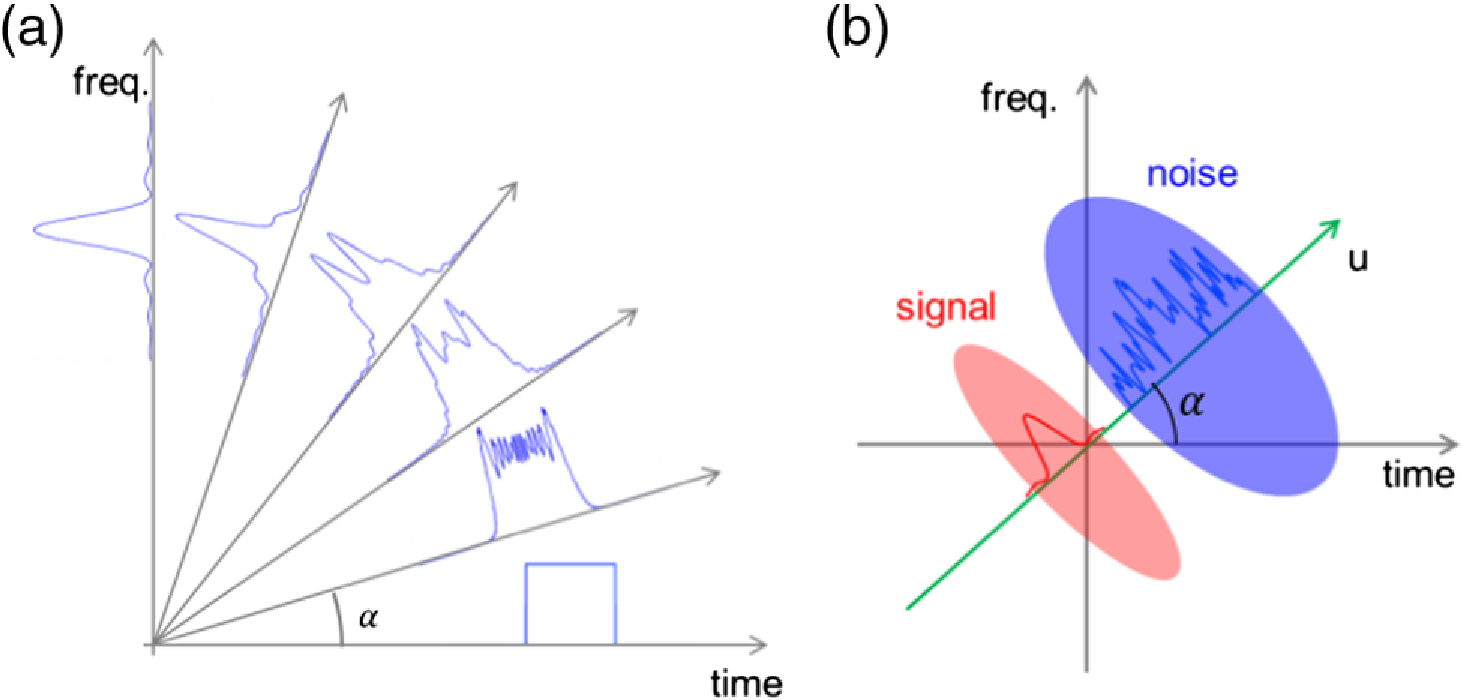
\includegraphics[width=1\textwidth]{FrFT_optica.jpg}
\end{figure}
Fractional Fourier Transform (FrFT) is a parameterized generalization of the FT. The FrFT transforms the signal from one basis to another basis between real and frequency space depending on the parameter a. The Fractional Fourier Transform of order a of a signal f is defined as:
\begin{equation}
f_{a}(x) = \int_{-\infty}^{\infty}K_{a}(x,x^{'})f(x^{'})dx^{'}
\end{equation}
where the convolution kernel is given by:

\begin{multline*}
	K_{a}(x,x^{'}) = \sqrt{\frac{1-icot(\alpha)}{2\pi}}*\\exp(i0.5(x^{2}cot(\alpha)-2xx^{'}csc(\alpha)+x^{'}cot(\alpha)))
\end{multline*}
where $\alpha = \frac{\pi a}{2}$\\ 
When a is an odd/even multiple of $\pi$, the convolution kernel reduces to:
\begin{equation}
	K_{a}(x,x^{'}) = \delta(x\pm x^{'})
\end{equation}
which just means that a rotation by odd multiple of $\pi$ is a parity operation and a rotation by an even multiple of $\pi$ is an identity operation. When $\alpha$ is $\frac{\pi}{2}$, the FrFT reduces to the familiar Fourer Transform. 

While we won't derive it here, Fresnel propagator is an integral transform that can be interpreted as a Fractional Fourier transform followed by a phase factor correction\cite{Hanna2011}. 

The FrFT itself can be seen as a specific case of a class of three parameter integral transforms known as Linear Canonical Transforms\cite{Hennelly05}. The LCT for the parameters $\alpha, \beta, \gamma$ is defined by 

\begin{multline*}
    	u_{\alpha, \beta, \gamma} = L_{\alpha, \beta, \gamma}{u(x)}(x^{'}) = \\ exp(\frac{-j\pi}{4})\sqrt{\beta}\int_{-\infty}^{\infty}u(x)exp[j\pi(\alpha x^{2} - 2\beta xx^{'} + \gamma x^{'2})]dx 
\end{multline*}
The LCT can be described by an abcd matrix which transform the Wigner Distribution as $W(x,k) \rightarrow W(ax+bk,cx+dk)$ with relations between a,b,c,d that limiting them to three degrees of freedom \cite{Hennelly05}. 

Thus, the LCT is a rotation in phase space from unprimed to primed co-ordinates given by \cite{Hennelly05} :
 \begin{equation}
	\begin{bmatrix}
	x^{'}\\
	k^{'}
	\end{bmatrix} = 
	\begin{bmatrix}
	a & b \\
	c & d
	\end{bmatrix}
	\begin{bmatrix}
	x\\
	k
	\end{bmatrix}
\end{equation}
The Fresnel transform is now described by the matrix \cite{Hennelly05} : 
\begin{equation}
    	\begin{bmatrix}
		a & b \\
		c & d
	\end{bmatrix}
	=
	\begin{bmatrix}
	1 & \lambda z \\
	0 & 1
	\end{bmatrix}	
\end{equation}
The Discrete Linear Canonical Transform (DLCT) can be implemented by "decomposition" into a set of LCT's as two LCT's can be cascaded together\cite{Healy2016}.  

\begin{figure}
\label{fig: DLCT_graphic}
\caption{Phase-Space representation of two algorithms for computation of the DLCT in terms of efficient operations (viz. Fourier Transform and Chirp Transform)\cite{Healy2016}} 
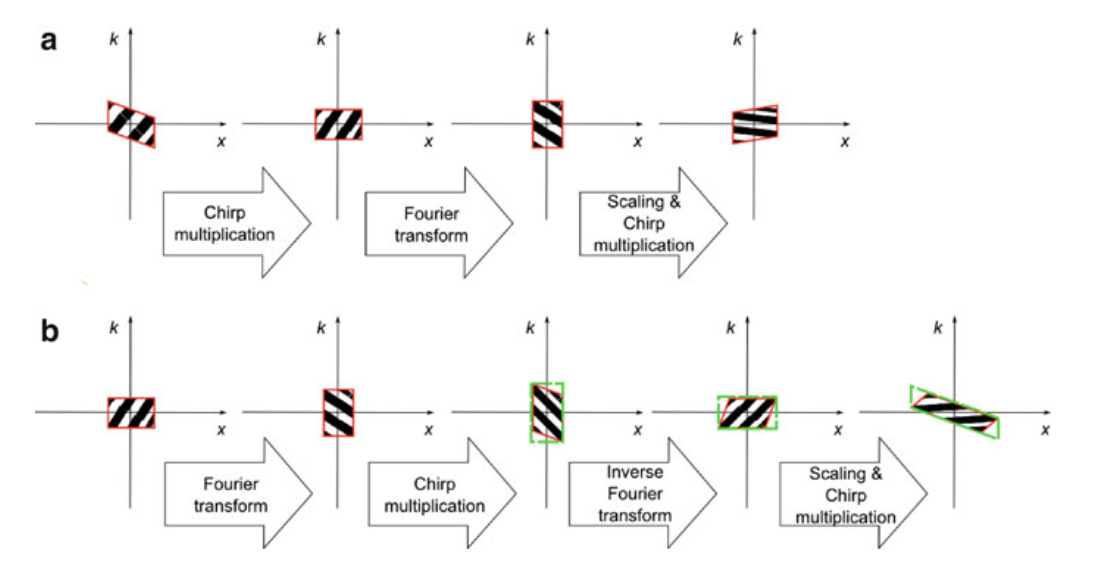
\includegraphics[width=1\textwidth]{DLCT_implementation.png}
\end{figure}
The task of finding efficient numerical algorithms for the evaluation of both the general and specialized cases of (Discrete) FrFT and (Discrete)LCT is an active field \cite{BULTHEEL2004182,Koç2016} and we hope that the X-ray wave propagation community can benefit from the latest research there. \\
\todo{VINCENT/DAVID: Review it!}


\section{Software packages}
\label{ch: packages}

We summarize here the software tools that implement the free-space wavefron propagators discussed in this paper. 

PyNX \todo{complete and check: VINCENT} \cite{Favre-Nicolin:hx5119} (Python tools for Nano-structures Xtallography) can be used for coherent X-ray imaging simulation and analysis: i) coherent diffraction imaging (CDI), Ptychography, Wavefront propagation, near field and far field techniques; and ii) Fast scattering calculations from large number of atoms and reciprocal space positions. PyNX is fully optimised to use Graphical Processing Units (GPUs), using either CUDA or OpenCL, to provide fast calculations with 1 to 3 orders of magnitude speedup compared to standard processor calculations. The propagators available in pyNX are: 
\begin{itemize}
    \item Near field propagation, based on Eq.~\ref{eq: Fresnel propagation in convolution form}
    \item Near field propagation with magnification, based on Section~\ref{subch: zoom}
    \item Far field propagator
    \item \inred{...}
\end{itemize}


SRW \todo{complete and check: OLEG} \cite{Chubar1998} (Synchrotron Radiation Workshop)is a software package to make a wide range of simulations of synchrotron radiation of arbitrary configurations as well as standard bending magnets, wigglers and undulators, and propagates it along a beamline composed by different kind of elements (slits, mirrors, gratings, real and ideal lenses, etc.). It can perform simulations on partially coherent synchrotron beams using a ``multi-electron'' method that allows to create, propagate and score radiation created from single electrons with initial conditions sampled by Monte Carlo from the statistical distribution of the electrons in the storage ring (Twiss parameters). The propagators available in SRW are: 
\begin{itemize}
    \item Standard, based in Eq.~\ref{eq: Fresnel propagation in convolution form}
    \item Quadratic Term, based in Sec.~\ref{subch: semianalytical}
    \item Quadratic Term Special, based in Eq.~XX
    \item From Waist, based in Eq.~XX
    \item To Waist, based in Eq.~XX
\end{itemize}

WOFRY \todo{complete and check: LUCA} \cite{Wofrygit} (Wave Optics FRamework in pYthon) is a python library that implements a framework for waveoptics calculations. It contains a threefold functionality: i) it provides a generalization (or abstraction) of a software tool for wave optics, combining the component definitions with the abstract declaration of wavefronts and propagators, ii) it defines a mechanism for interfacing a wave optics code (e.g., SRW, WISE etc.) in it, a first step for creating high level user interfaces in OASYS \cite{oasys}, and iii) it provides native implementations of simple wavefronts (e.g., plane waves, spherical waves, Gaussian sources) and propagators for prototyping optical systems.
The propagators available in WOFRY are: 
\begin{itemize}
    \item Fresnel, based in Eq.~\ref{eq: Fresnel propagation in convolution form}
    \item Fresnel Convolution, based in Eq.~\ref{eq: Fresnel propagation in convolution form} \inred{(using numpy.convolution)}
    \item Fraunhoffer, based in Eq.~XX
    \item Integral, non-fourier calculation of integral, based in Eq.~\ref{eq: discretefresnel} (2D) or Eq.~\ref{eq: discretefresnel1D} (1D)
    \item Fresnel Zoom XY, based on Sect.~\ref{subch: zoom}
\end{itemize}

\todo{SAJID: Define your library...}
The propagators available in XWP are: 
\begin{itemize}
    \item \inred{...}
\end{itemize}

This paper concerns only the methods, algorithms and implementation of free-space propagators in these codes. Certainly the functionality of each code goes beyond of the simple propagation in vacuum and we refer to the references and documentation of each code for further details. Moreover, similar methodologies can be found in several other software tools (e.g., WISE \cite{wise}, RAY \inred{REF}, McXtrace \cite{mcxtrace}, ...) and also in the calculations presented in several publications \inred{Osterhoff, ...}.


\section{Non-Fourier Fresnel propagator implementation}
\label{ch: non-fourier-propagators}

In the previous section an exact solution to the boundary-value problem of propagation of a wavefront between two parallel planes in free space in the paraxial approximation was found. At this point, it is necessary to recast the expression in a way that let us solve it numerically. In Subsection~\ref{subch: discretization} we discuss the discrete sampling of the wavefronts and the expressions of the Fresnel propagator as finite sums in order to be implemented in a computer. We illustrate the implementation of a simple Fresnel propagator in 1D and apply it to compute the scholar case of an apertire illuminated by a plane wave. We use this example to illustrate the artifacts that one may obtain depending on how the wavefronts are discretized.


\subsection{Wavefront and propagator discretization}
\label{subch: discretization}
\todo{RC: Maybe a discussion similar to the one presented here: https://doi.org/10.1364/JOSAA.31.001832 would be interesting. Sampling guidelines are also discussed on this work. There is another interesting work from the same group here: https://doi.org/10.1364/JOSAA.31.000755}

A complex wavefront $U(x,y,z=z_0)$ in a plane perpendicular to the $z$ propagation direction at $z=z_0$ can be represented in a computer by giving the values of $U$ on a grid that must be finite and discrete. Let us call ${x_0,x_1,...,x_{N_x-1}}$ the discrete values for the (horizontal) spatial coordinates and similarly  ${y_0,y_1,...,y_{N_y-1}}$ for the (vertical) component. The point $(x_i,y_j)$ with $i \in [0,N_x)$ and  $j \in [0,N_y)$ is a sampled point of indices $(i,j)$. The 2D array of evaluated points $U(x_i,y_j) \equiv U_{ij}$ is the numeric representation of the wavefront. This representation is limited by two factors: finite window size and finite step size. The numeric wavefield is defined in a finite domain or window of dimension $(x_{N_x-1}-x_0) \times (y_{N_y-1}-y_0)$. This domain must be large enough to contain all points where the wavefront disturbance is different from zero. Obviously it is impossible to fully describe a plane wave ($U(x,y)$=Cte) that, in the numerical representation will always be clipped in a finite domain. The grid must be dense enough to follow with enough detail all the variations of $U$. This is also a big limitation because $U$ (in particular its phase) can change very rapidly versus $x$ or $y$ in waves that are strongly convergent or divergent, as it usual when applying mirrors, lenses or other focusing elements. This limitation will be discussed in detail. 

If one wants to calculated the propagated disturbance one has to apply Eq.~\ref{eq: usualfresnel}. Let us call, like in Eq.~\ref{eq: usualfresnel}, with primes $(x^\prime_i,y^\prime_j)$ the discretization of the spatial of the source wavefront at $z=0$. The propagated disturbance at a point of coordinates $(x,y)$ at the plane $z=\Delta z$ can be calculated approximately by discretizing the integrals into sums: 
\begin{equation}\label{eq: discretefresnel}
 U(x,y) = \frac {e^{ik\Delta z }}{ i \lambda \Delta z} \sum_{i=0}^{N_x-1}  \sum_{j=0}^{N_y-1} U(x^\prime_i, y^\prime_j, 0) e^{i \frac{k}{2 \Delta z} [(x - x_i^\prime)^2 + (y - y_j^\prime)^2]} \delta_i x^\prime \delta_j y^\prime
\end{equation}
where $\delta_i x^\prime = x^\prime_{i+1} - x^\prime_i$ and similarly for $y$. In many cases the abscissas grid is homogeneous with constant step $\delta_i x^\prime = \delta_x$. Note that for calculating the propagated disturbance at a single point on the detector plane one has to add the contribution of each point of the source multiplied by a phase that depends on the distance of that point to the detector point. Therefore the number of operations is of the order of $N_{x^\prime}  N_{y^\prime}$ for a single point on the detector. If, as usual, one wants to calculate the disturbance in a grid in the detector plane, the numbers of operation would be $N_{x^\prime}  N_{y^\prime} N_{x}  N_{y} \sim N^4$. 
The reduction of Eq.~\ref{eq: discretefresnel} to 1D is trivial:
\begin{equation}\label{eq: discretefresnel1D}
 U(x,y) = \frac {e^{ik\Delta z }}{ \sqrt{i \lambda \Delta z}} \sum_{i=0}^{N_x-1}  U(x^\prime_i, 0) e^{i \frac{k}{2 \Delta z} (x - x_i^\prime)^2 } \delta_i x^\prime
\end{equation}


Fig.~\ref{fig: aperture_1D} shows the propagated disturbance at a distance $D$ of a plane wave in the near field.

\begin{figure}
\label{fig: aperture_1D}
\caption{Propagation of a plane wavefront of photon energy 10 keV clipped by a slit in the near field (propagation distance 75$\mu$m). Window size $w$=5$\mu$m, aperture=$w$/4, number of pixels: 2048. 
The results shown used XWP and WOFRY giving identical results. 
\ingreen{ https://github.com/srio/propagation-free-space/blob/master/examples/aperture\_1D.py}
}
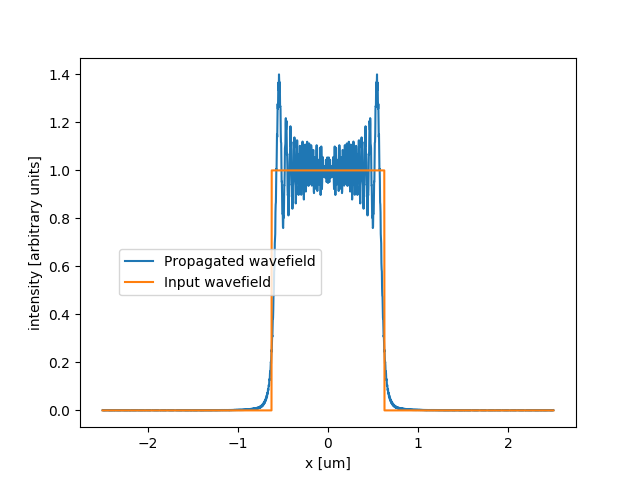
\includegraphics[width=1\textwidth]{aperture_1D.png}
\end{figure}


\subsection{Replicas and aliasing}

Figure~\ref{fig: aperture_1D} show a simple example of propagating a simple field (plane wave) by a distance $D$. The sampling parameters (window size, number of points) have been "adequately" selected in order to obtain "reasonable" results. One can experiment playing with these parameters to illustrate how critical is the right selection of the parameters. Let us increase the pixel size $d_p=w/(N-1)$ by a factor of 2, or in other words reduce the number of pixels by a factor 2. The result in Fig.~\ref{fig: aperture_1D_replica}a shows that although the main diffracted feature is present (with a lower resolution) some unwanted replicas are present at periodic distances from the main centered feature. These are consequences of the inadequate sampling of the wavefield (undersampling). This is explained by the Whittaker-Shannon sampling theorem that imposes a sufficient condition related to the Nyquist frequency for representing (sampling) continuous function by a discrete collection of points. Instead of using this theorem to explain the results observed in Fig.~\ref{fig: aperture_1D_replica} we can think in a more "optical" approach. The fact that we sample our continuous wavefield over a grid of points with periodicity $d_p$ is similar that we superpose to our field a diffraction grating of this ruling period. As a result, one obtains the zeroth order diffraction (main diffracted feature) overlapped by non-zero diffracted orders (our replicas). A simple application of the grating equation $\sin \theta = m \lambda / d_p $ gives the angular position $\theta$ of the different orders $m$. The position of the replica are at $m \theta D$. Using parameters of Fig.~\ref{fig: aperture_1D_replica} one obtains $\theta D= 1.9 \mu m$ in good agreement with the numerical results. 

Replicas can be avoided by increasing the sampling (reducing $d_p$) or by isolating the main feature at the image plane, if the replica are well separated. The situation becomes worse if the selected wavefront sampling produces an overlapping of the replicas, thus completely distorting the expected result. Fig.~\ref{fig: aperture_1D_replica}b shows the effect of further reduce the number of points bu a factor of 2. This overlapping effect of the replicas is called {\it aliasing} and it is an artifact due to the numerical simulation, in particular a bad sampling. 

In the examples shown we have chosen the input and output windows of equal size, as well as the same number of pixels (points) in the input and output planes. This is not required as Eq.~\ref{eq: discretefresnel1D} permits to sample independently the input and output fields. Moreover, the grid chosen is uniform. This situation could be relaxed. If so, the lack of periodicity could be beneficial for avoiding replicas. \todo{example?}


\begin{figure}
\label{fig: aperture_1D_replica}
\caption{Propagation of a plane wavefront of photon energy 10 keV clipped by a slit in the near field (propagation distance 75$\mu$m). Window size $w$=5$\mu$m, aperture=$w$/4, number of pixels: 1024 (left) and 512 (right). \ingreen{aperture\_1D\_replicas.py}
}
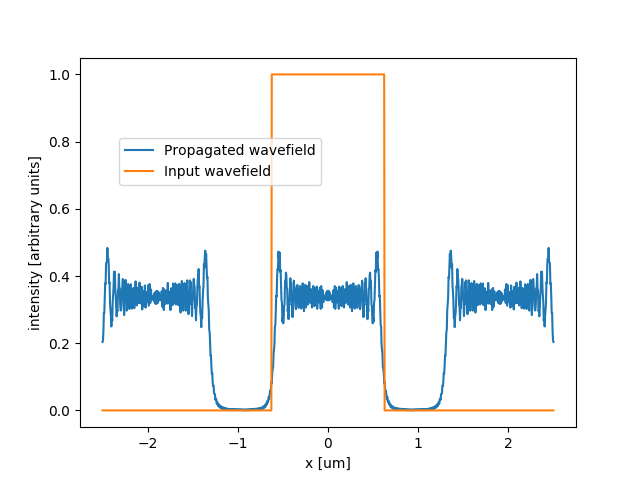
\includegraphics[width=0.45\textwidth]{aperture_1D_over2.png}
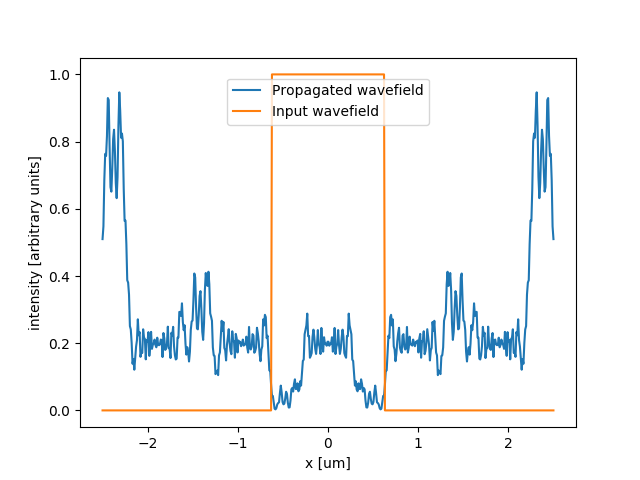
\includegraphics[width=0.45\textwidth]{aperture_1D_over4.png}
\end{figure}


The system simulated in Fig.~\ref{fig: aperture_1D} refers to  the Fresnel diffraction of a plane wave clipped by a rectangular slit. The diffracted wavefield can in this case be calculated analytically and the result is expressed in terms of the Fresnel integrals (see Ref.~\cite{goodmanfourier}).  Figure~\ref{fig: aperture_1D_analytical} shows the central part of the pattern in Fig.~\ref{fig: aperture_1D} calculated with WOFRY (integral) and XWP (exact\_numba) and compared to the analytic result. 


\begin{figure}
\label{fig: aperture_1D_analytical}
\caption{Comparison of the central part of the pattern in Fig.~\ref{fig: aperture_1D} calculated with XWP (exact\_numba) and WOFRY (integral) and compared to the analytical results.
}
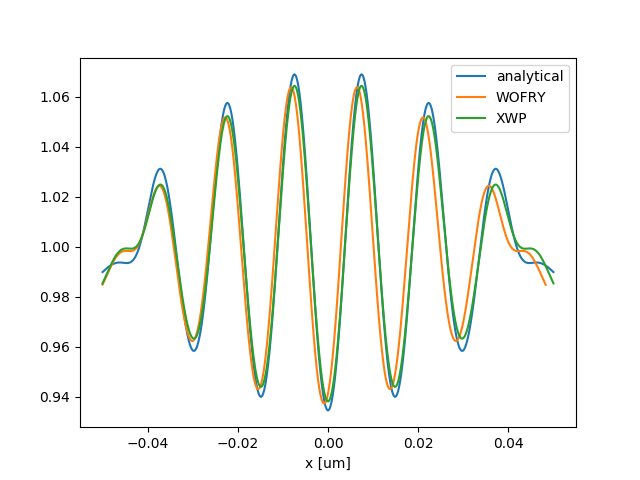
\includegraphics[width=1\textwidth]{aperture_1D_analytical.png}
\end{figure}


\section{Fourier Fresnel propagator implementation}
\label{ch: fourier-propagators}


If we consider a wavefront sampled in $N \times N$ pixels (being $N > 10^3$), when calculating the 2D integrals to propagate the wavefront to another plane with the same resolution, we need approximately $N^2\cdot N^2 \approx 10^{12}$ operations. This implicate the necessity of a great amount of storage and calculations not feasible for normal computers. When performing the same calculations taking advantage of the theory of Fourier optics, one $FFT$ requires $\approx N^2 \log_2 N \approx 10^7$ operations \cite{Marshall:1992:CVM:129191}. This is the reason why we seek for a form that let us exploit such powerful tool. 

The expression of the Fresnel propagator in Eq.~\ref{eq: Fresnel propagation in convolution form} is suitable to be calculated numerically with the use of Fast Fourier Transform algorithm ($FFT$) simply swapping the Fourier transform operator $\mathcal{F}\big\{\big\}$ with the discrete Fourier transform one $FFT$, taking into account the sampling conditions that are discussed later. That is, one arrives at \todo{explain the kernel is changed to account for different definition of the fourier transform}
\begin{equation}\label{eq: standard propagator}
U(x, y, \Delta z)= \frac{e^{ik\Delta z}}{2\pi} FFT^{-1}\Big\{ FTT\big\{U(x, y, 0)\big\} \times e^{-i \pi \lambda \Delta z (f_x^2 + f_y^2) \Big\}
\end{equation} 
This is the standard implementation of the Fresnel propagator using two FFT implemented in most computer codes for synchrotron radiation. The use of FFT is not restricted to this propagator. Indeed, Eq.~\ref{eq: before fraunhoffer} represents the Fresnel propagator as Fourier transform of the distrurbance $U$ multiplied by a quadratic term. This allows to compute the Fresnel propagator using a single FFT \todo{explain why this is not so popular and is not used in synchrotron radiation (as far as I know...)}. The in the Fraunhofer regime, this quadratic phase is approximated by one so the propagated disturbance is just the Fourier transform of the unpropagated one, a phenomenon that is very well known in many fields of Physics. 


\subsection{Example of 2D rectangular and circular apertures. Comparison with analytical results.}
\label{subch: apertures}

The near field calculation presented in Fig.~\ref{fig: aperture_1D_analytical} is calculated now in 2D for both square and circular apertures, applying the Fresnel propagator that uses FFT (Eq.~\ref{eq: Fresnel propagation in convolution form}. The calculation results using ``SRW standard propagator'' is presented in Fig.~\ref{fig: SRW aperture}. 
\begin{figure}
\label{fig: SRW aperture}
\caption{Propagation of a plane wavefront of photon energy 10 keV in the near field (propagation distance 75$\mu$m) clipped by a rectangular slit (left) and circular slit (right). Window size is $w$=5$\mu$m, the aperture height and width or diameter is $w$/4, number of pixels: 2048$\times$2048. The bottom row show the profiles at $y=0$. These calculations have been done with SRW. \todo{bigger graphics?}
}
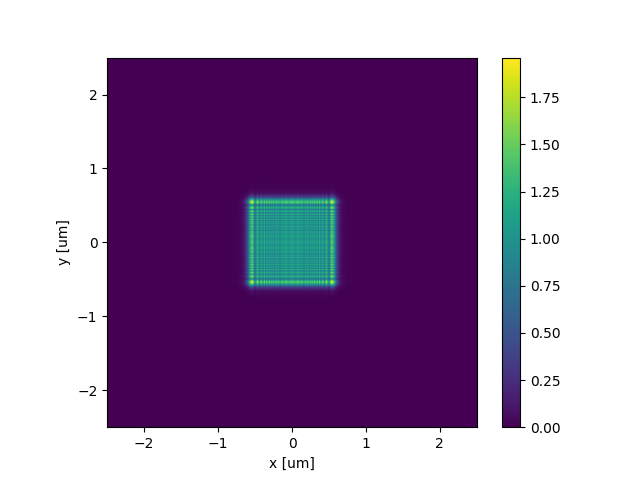
\includegraphics[width=0.45\textwidth]{aperture_2D_rectangular_srw.png}
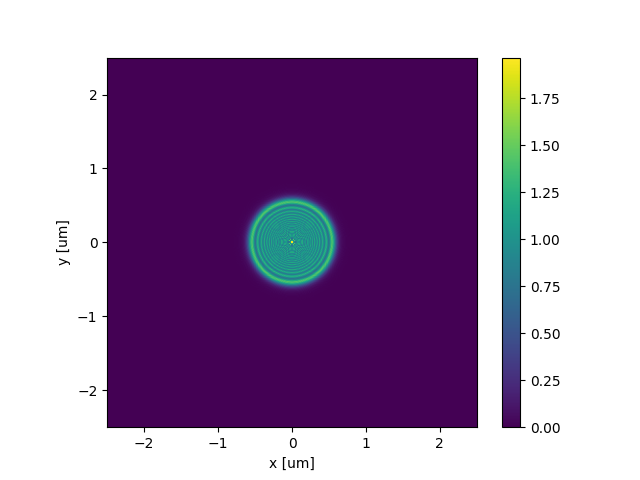
\includegraphics[width=0.45\textwidth]{aperture_2D_circular_srw.png}
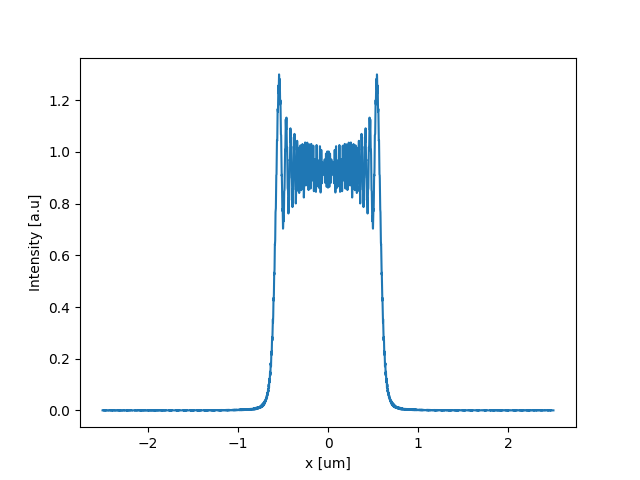
\includegraphics[width=0.45\textwidth]{aperture_2D_rectangular_profile_srw.png}
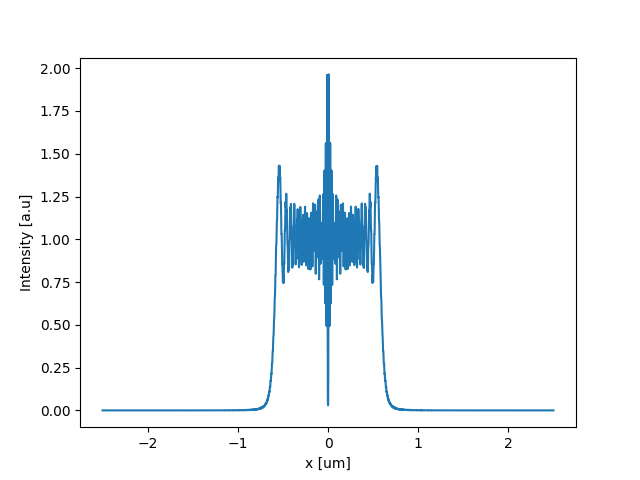
\includegraphics[width=0.45\textwidth]{aperture_2D_circular_profile_srw.png}
\end{figure}
Following the same scenario as done for 1D calculations, we want now to compare in detail the results of the different packages presented here with the analytical results. Fig.~\ref{fig: 2D aperture comparison} shows a zoom of the central part of the profile at $y=0$ in Fig.~\ref{fig: SRW aperture} calculated with different libraries. 
\begin{figure}
\label{fig: SRW aperture comparison}
\caption{The central part of the diffraction pattern profiles at $y=0$ for a rectangular aperture (a) and circular aperture (b) in Fig.~\ref{fig: SRW aperture} with 4096$\times$4096 pixels. Results of different software packages are compared with the analytical results.\todo{calculate with pyNX and XWP}
}
a)
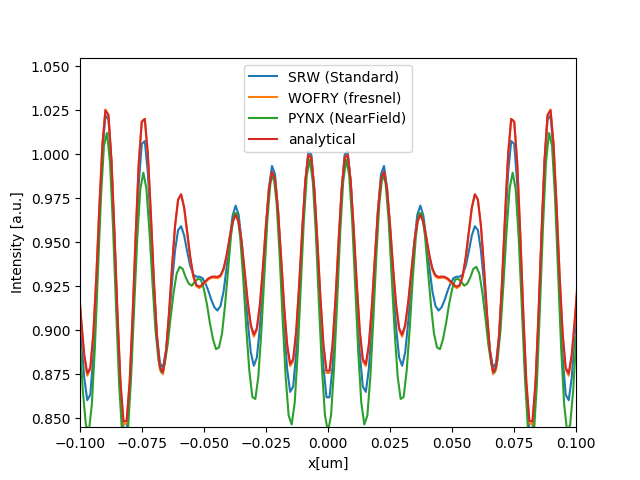
\includegraphics[width=0.45\textwidth]{aperture_2D_rectangular_profile_comparison.png}
b)
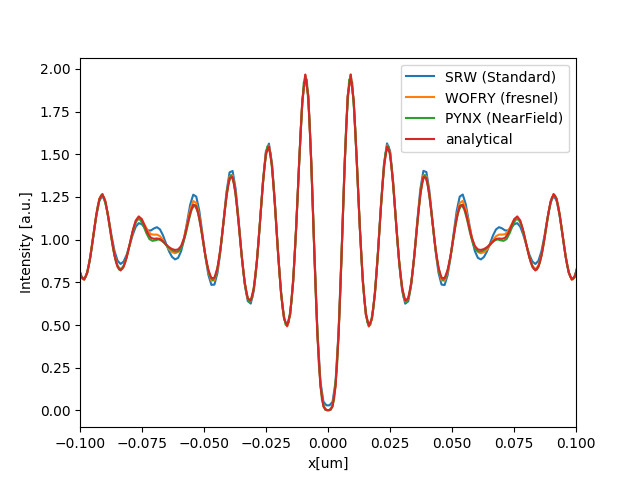
\includegraphics[width=0.45\textwidth]{aperture_2D_circular_profile_comparison.png}
\end{figure}


\todo{ Look at the phase. Discuss Control parameters: 
\begin{enumerate}
\item Window size
\item Pixel size
\item Number of points (power of 2?)
\item odd or even number of points
\end{enumerate}
 
}

\todo{discuss one FFT Fresnel propagator implementation and Fraunhofer implementation???}

\section{Other propagators for diffraction by convergent and divergent wavefronts}
\label{ch: propagators convergent}

This is the case for very converging or divergent beams where wavefront curvature is high so the phase oscillates very rapidily. This case is often found in synchrotron beamlines which usually contain focusing elements. In these cases, the number of points required to sample correctly the phase over the whole window impractical. Moreover, the size of the source and image windows, which are equal when applying the ``standard'' propagator, appear to be very different in real life when the image is close to the focal position or waist. To deal with these cases, some tricks must be found. There are discussed in the next chapter.

\subsection{The Fresnel scaling theorem.}
\label{subch: Fresnel scaling}
\todo{DAVID: please review and complete}
It can be shown that the diffraction pattern at a given image position of an object illuminated by a spherical wavefront is the same (except for a scaling factor) than the diffraction pattern of the same object illuminated by a plane wave at another given distance. 
The interest of this theorem is when one wants to compute the diffraction of an object illuminated by a highly converging or divergent wavefront, where the problem of phase sampling is important. It can be solved by simulating the corresponding problem of illumination with a plane wave where the sampling phase problem is not found.

In Appendix \ref{appendix_scaling} a full derivation of the Fresnel scattering theorem is presented, following \cite{paganin_book} but including the phase in the result. Let $U(x,y,0$ the incident field consisting of either a plane or spherical wave scattered by an object (for example, clipped by an aperture). Let call $U^R(x,y,z)$ the disturbance propagated at a distance $z$ when the phase of the incident wave corresponds to a spherical wave and $U^\infty(x,y,z)$ for a plane wave. The theorem states that the disturbance by the spherical wave at a distance $z=\Delta$ is ``similar'' to the image produced by a plane wave at another distance $\Delta/M$. ``Similar'' means spatially spaced and with a constant phase term.

\begin{equation}
	U^{(R)}(x, y, \Delta)= \frac{1}{M} e^{\big[ik\Delta \big({1-\frac{1}{M}}\big)\big]} e^{\big[\frac{ik}{2\Delta}(x^2+y^2)\big(\frac{M-1}{M}\big)\big]} U^{(\infty)}\Big(\frac{x}{M}, \frac{y}{M}, \frac{\Delta}{M}\Big)
\end{equation}


\subsection{Semianalytical treatment of spherical phase}
\label{subch: semianalytical}

\todo{RAPHAEL to write this section, OLEG to review it.}

We introduce here one of the the methodology used in some of the propagators available in SRW. The goal is to write the incident disturbance $U(x,y,0)$ as a product of a ``precursor'' field $U^P(x,y,0)$ times a ``toroidal phase'' $Y^T(x,y,0)$ in such a way that the precursor field is treated numerically and does not present a converging behavior or highly oscillating phase, and the toroidal field is treated analytically as additional phase terms. One can write: 
\begin{equation}
\begin{aligned}
U(x,y,0) =& U^P(x,y,0) U^T(x,y,0); \\
U^T(x,y,0;R_x,R_y,x_c,y_c) =& e^{ik [\frac{(x-x_c)^2}{2 R_x} + \frac{(y-y_c)^2}{2 R_y}]}
\end{aligned}
\end{equation}
where $R_x$ and $R_y$ are the meridional and sagittal radii of the toroidal front, and $(x_c,y_x)$ is the center of the toroid. The precursor field is $U^P=U U^R(-R_x,-R_y,x_c,y_c)$. 
In appendix \ref{appendix_srw} it can be shown that the problem reduces to a convolution problem of the precursor field $U^P$ affected by a phase $P$ with a \inred{new?} kernel $K$, and the result affected by a global phase $P^G$: 
\begin{equation}
\label{eq: srw in convolution form}
U(x, y, \Delta) = P^G \mathcal{F}^{-1}\Big[\mathcal{F}\big[U^P P \big] K \Big]
\end{equation}
where \todo{copy here $P^G$, $P$ and $K$ to be deduced in Appendix \ref{appendix_srw}. Cite and comment Ref.~\cite{wyrowski}}


\subsection{The Zoom Propagator}
\label{subch: zoom}

\todo{GIOVANNI, LUCA, please extend and review}

This section presents the formalism used for a propagator that makes possible to calculate thye propagated field in a ``zoomed'' window, thus permitting optimizing the wavefront sampling in cases for propagating highly convergent or divergent wavefronts. The work here follows the work in the book of J.D. Schmidt \cite{schmidt} extended for including different zoom factors in horizontal and vertical. 

In appendix \ref{appendix_zoom} it can be shown that the problem reduces to a convolution problem of the precursor field $U^P$ affected by a phase $P$ with a \inred{new?} kernel $K$, and the result affected by a global phase $P^G$: 
\begin{equation}
U(x, y, \Delta) = P^G \mathcal{F}^{-1}\Big[\mathcal{F}\big[U^P P \big] K \Big]
\end{equation}
where
\begin{equation}
P^G =  \frac { e^{ik\Delta z }}{\sqrt{m_x m_y} }e^{i \frac{k}{2 \Delta z} [\frac{m_x - 1}{m_x}x_2^2 + \frac{m_y - 1}{m_y}y_2^2]}  \\
\end{equation}
\begin{equation}
P = e^{i \frac{k}{2 \Delta z} [(1-m_x)x_1^2 + (1-m_y)y_1^2]} \\
\end{equation}
\begin{equation}
K = e^{-i \pi \lambda \Delta z (\frac{f_x^2}{m_x} +\frac{f_y^2}{m_y})}
\end{equation}

Note that setting one magnification $m_x=m_y=1$ one obtains the standatd Fresnel propagator (Eq.~\ref{eq: numerical convolution form of angular spectrum}), with  $P=1$, $P^G=\exp(i k \Delta z)$  and $K= e^{-i \pi \lambda \Delta z (f_x^2 +f_y^2)}$.


\subsection{Example: propagate a collapsing spherical wavefront to its focal plane}
\label{subch: aperture converging}

We study here the focal pattern produced by a highly converging wavefront clipped by a rectangular aperture. For that, a spherical wave of radius $R=-10$ cm of wave field $U(x,y,0) = \exp(i k (x^2 + y^2) / (2 R)$ clipped by a square slit, thus  zero outside a domain $-D/2\le x\le D/2$, domain $-D/2\le x\le D/2$. The photon energy is $E=10$ keV and $D=100 \mu$m. 
This field is propagated to the focal position, thus $\Delta z$=10 cm.This situation may represent an over-simplification of the last step of a real nonofocusing beamline \cite{ID16A}, where a highly coherent beam represented by a plane wave enters in a  Kirkpatrick-Baez system that i) clips the wavefront because of its limited numerical aperture, and ii) converts the plane wave into an approximately spherical wave converging to the focal position.

The case of diffraction of a collapsing spherical wave clipped a square slit can be calculated analitically useng the Fresnel propagator thus assuming paraxial approximation. As shown in Appendix~\ref{appendix_collapsing}, the diffracted intensity distribition at the focal plane is
\begin{equation}
    |U(x,y,z=\Delta z)|^2 = \left( \frac{2 k D^2}{\pi \Delta z}\right)^2 sinc^2\frac{k x D}{2 \Delta z} sinc^2\frac{k y D}{2 \Delta z}
\end{equation}
with $sinx(x)=\sin(x}/x$. Note that this pattern is the same (except for the scaling factor) as the pattern produced by a plane wave at $\Dz=\infty$ (in the far field using the Fraunhofer approximation). Fig.~\ref{fig: slit 2D converging} shows the results of some numerical calculations using WOFRY(zoom), SRW(quadratic), \inred{add more...} compared with the analytical result. The agreement is very good in general, thus the data are presented in log scale to better appreciate small differences.  

\todo{Discuss the phase. May be illustrate the Gouy phase?}

\begin{figure}
\label{fig: slit 2D converging}
\caption{Propagation of a spherical converging wavefront ($R=-10$ cm) of photon energy 10 keV to the focal position at a distance $\Delta z = 10$ cm. The window size $w=100 \times 100 \mu m^2$, number of pixels: 2048$\times$2048. The results shown have been calculated with SRW (semianalytical propagator) and WOFRY (zoom propagator). \ingreen{aperture\_2D\_converging.py} \inred{Interestingly this picture changed after upgrading my Mac OS... In particular SRW result. Now the agreement is much better!! Why??}
}
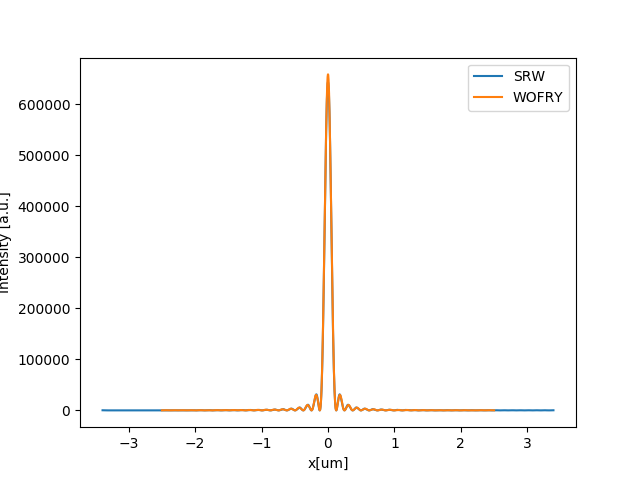
\includegraphics[width=0.95\textwidth]{aperture_2D_converging.png}
\end{figure}



\section{Validity conditions}
\label{ch: validity}

It has been shown that undesampling the source cause replicas in the image (see Fig.~\ref{fig: aperture_1D}). When using FFT the situation becomes even more dangerous and also aliasing may appear. In the previous sections we discussed how a correct sample of the wavefront is essential to avoid unwanted results. The question if what is the correct sampling of the wavefront is not easy to answer on a-priori basis. Therefore, in many cases one uses iterative simulations until obtaining some ``realistic'' results (some cleam image, without replicas and with a good resolution of the physical features in the image. This practical approach may lead to errors, as sometimes it is not easy to distinguish betwen features that are physical or are numerical artifacts. In many cases, using the standard propagators, one arrives to the limit of the possibilities of the computer memory that makes impossible to increase resolution (increment the grid size) more and more.

In this section we formalize the conditions for good sampling of the phase in the implementation of the numerical propagators. We follow the ideas of \cite{goodmanfourier} and results in \cite{schmidt}, \cite{pirro} and PYNX code.  

Let us consider a quadratic phase term $\exp(i A x^2)$. The condition for ``good sampling'' is:

\begin{equation}
\frac{1}{2 \pi} \frac{\partial}{\partial x}(A x^2) = \frac{1}{2 \delta_x},
\end{equation}
expressing the spatial coordinate $x_j=X_J \delta_x$ with $X_j = [-N/2,-N/2 -1, ..., N/2[$ (N even) or $X_j = [-(N-1)/2,...(N-1)/2[$ (N odd)
\begin{equation}
\frac{1}{2 \pi} \frac{1}{\delta_x} \frac{\partial}{\partial X}(A (X \delta_x)^2) = \frac{1}{2 \delta_x}
\end{equation}
\begin{equation}\label{eq: good sampling condition}
A \leq \frac{\pi}{N \delta_x^2}
\end{equation}

\begin{figure}
\label{fig: phase sampling}
\caption{Illustration of a good sampling (a) and bad sampling (b) of the real part of the function $f(x)=exp(i A x^2)$ with (a) $A$=20$< \pi / (N \delta_x^2)$ and (b) $A$=30$ > \pi / (N \delta_x^2)$ with $N=10$ and $\pi / (N \delta_x^2)$=25.4. 
}
a)
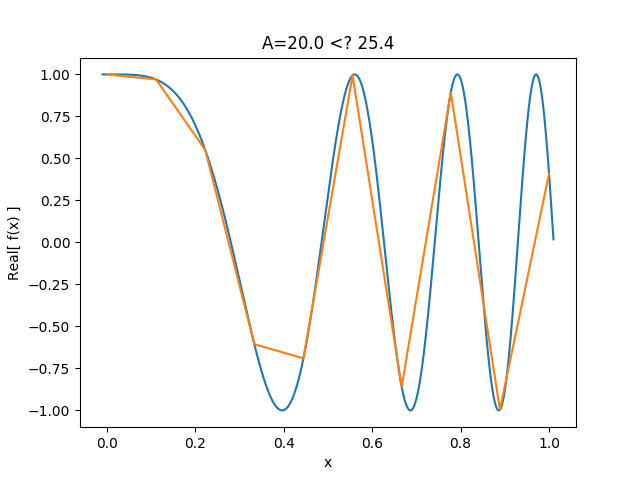
\includegraphics[width=0.45\textwidth]{sample_quadratic_phase_A20.png}
b)https://www.overleaf.com/18319766dfmqmnvnnpmk
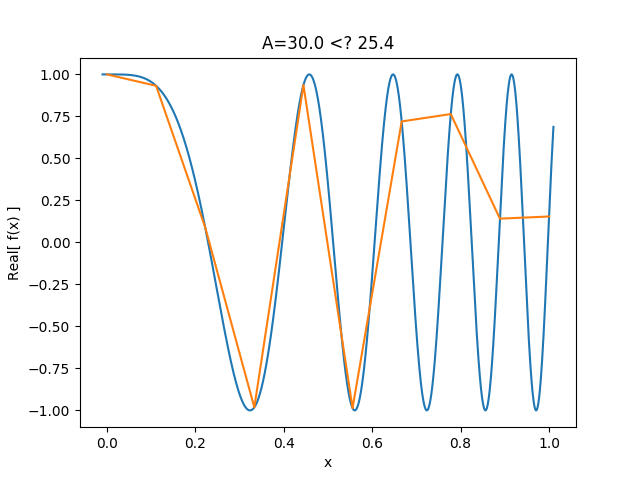
\includegraphics[width=0.45\textwidth]{sample_quadratic_phase_A30.png}
\end{figure}

The condition in Eq.~\ref{eq: good sampling condition} should be applied to all quadratic exponential phases in all propagators. Before applying it to the different propagators, we can conside the case when the incident wavefront has a strong curvature. Let us think in a 1D
field that can be factorised into some remaining field multiplied by a phase $\exp(i k x^2 /  (2 R_x))$. Applying the validity condition in Eq.~\ref{eq: good sampling condition}, one obtains the minimum affordable radius for correct sampling as a function of the wavelength and sampling conditions parameters $\delta_x$ and $N_x$
\begin{equation}
    R_x > \frac{N_x \delta_x^2}{\lambda}
\end{equation}

\todo{This condition is not satisfied by Fig.~\ref{fig: slit 2D converging}, It would need 4 times more pixels in H and also in V (16x) what is difficult...}

\subsection{The Fresnel propagator with two FFTs}
The standard propagator is implemented using Eq.~\ref{eq: standard propagator}. The kernel has a form $\exp(A x^2)$ where (using $f_{x,j}=X_j \delta_f$, $\delta_f = 1/(N_x \delta_x)$)
\begin{equation}
    -\pi \lambda \Delta z f_x^2 = 
    -\pi \lambda \Delta z \left(\frac{x}{N_x \delta_x^2} \right)^2 = A x^2 
\end{equation}
therefore the validity condition gives
\begin{equation}\label{eq: fresnel validity}
    \Delta z < \frac{N_x \delta_x^2}{\lambda}  = \frac{W^2}{N_x \lambda}
\end{equation}
being $W$ the window size ($W=N_x \delta_x$). Note that an increase of the number of points for a constant window will \inblue{reduce} the maximum allowed propagation distance. For incrementing $\Delta z$ one has to increase the window. 

For example, under the conditions of Fig.~\ref{fig: SRW aperture} ($N$=2048) and Fig.~\ref{fig: SRW aperture comparison} ($N$=4096) the condition \ref{eq: good sampling fresnel} is represented in Fig.~\ref{fig: fresnel validity}. Note also the maximum allowed propagation distance is in general very small, therefore this standard propagator is valid only in the near-field region. 


\begin{figure}\label{fig: fresnel validity}
\caption{Validity plot for the propagation distance applied to the cases of Fig.~\ref{fig: SRW aperture} ($N$=2048) and Fig.~\ref{fig: SRW aperture comparison} ($N$=4096).
}
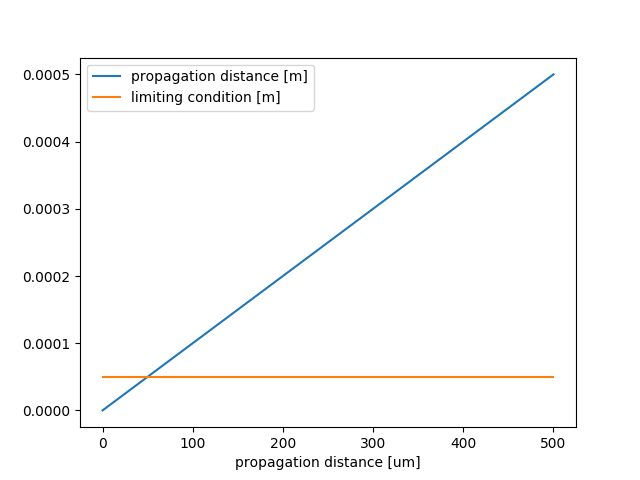
\includegraphics[width=0.95\textwidth]{fresnel_propagator_validity.png}
\end{figure}

\subsection{The Fresnel propagator with one FFTs}

Following Eq.~\ref{eq: fresnel2} the propagated field can be calculated by doing one-FFt of the unpropagated field multiplied by a quadratic phase: 

\begin{equation}
    U(x,y,\Delta z) = \frac{e^{i k \delta z}}{i \lambda \Delta z} FFT\left\{ U(x,y,0) e^{-i\frac{k}{\Delta z}(x^2+y^2)}\right\}
\end{equation}
Applying the validity condition to the exponential in the FFT, one gets: 
\begin{equation}\label{fig: fresnel2 validity}
    \Delta z > \frac{N \delta_x^2}{\lambda}.
\end{equation}
This equation is the contrary of what is found in Eq.~\ref{eq: fresnel validity}. For that reason the two-FFT Fresnel propagator is applicable in the "near field" whereas the one-FFT propagator is for the "far field". 

As discussed in \cite{Li}, the two analytically equivalent methods of Eqs.~\ref{eq: usualfresnel} and
\ref{eq: fresnel2} are useful in different regimes. In the one-FFT propagator, the input plane wavefield is multiplied by the real space propagator given in Eq.~XX. In the 2-FFTs propagator (convolution approach), the Fourier-transformed input plane wavefield is multiplied
by the reciprocal space propagator of Eq. XXX. The validity conditions indicate that the reciprocal space
propagator (two-FFTs) is slowly varying at shorter propagation distances, while the real space propagator (one-FFT) is slowly varying at longer propagation distances.

Figure~\ref{fig: far_field} shows a 1D calculation of the system presented in Fig.~\ref{fig: aperture_1D} but at a distance $\Delta z$=10 cm with N=5$\times$2048 pixels. The calculation and the analytical results are indistinguishable in the vicinity of the peak, but the tails present a different slope. Left: diffraction pattern close to the main peak. Right: large domain for the diffraction pattern where one can observe the differences in the slope of the tails.

\begin{figure}\label{fig: far_field}
    \centering
    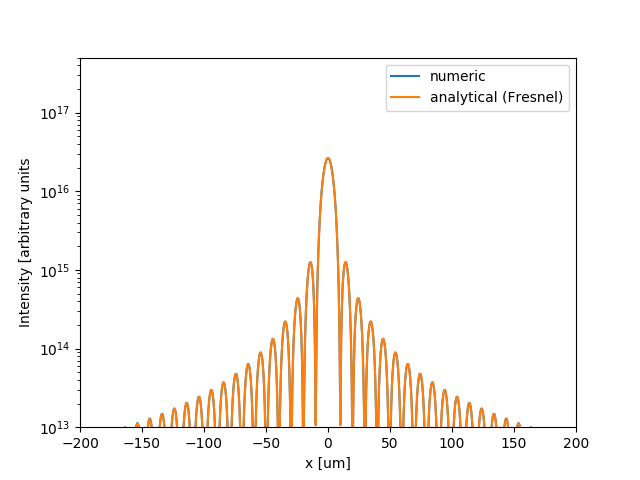
\includegraphics[width=0.45\textwidth]{far_field_a.png}
    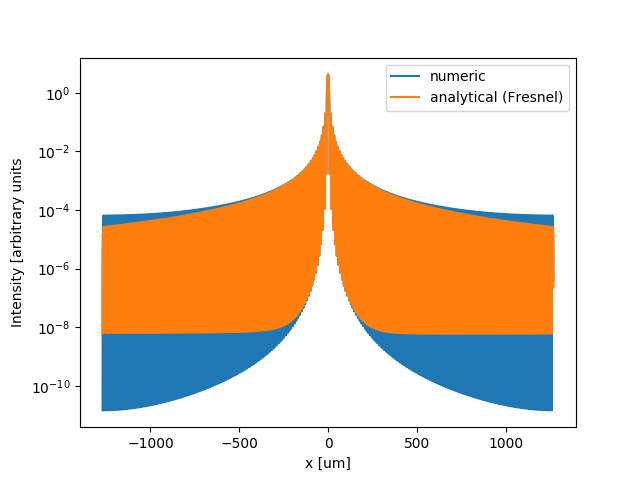
\includegraphics[width=0.45\textwidth]{far_field_b.png}
    \caption{Propagation of a plane wavefront of photon energy 10 keV clipped by a slit in the far field (propagation distance 0.1 m). Window size $w$=5$\mu$m, aperture=1.25$\mu$m, number of pixels: 5$\times$2048. }
\end{figure}

In the case of an incident wavefront with a curvature $R$, the validity condition becomes (see, e.g., \cite{schmidt})
\begin{equation}
\Delta z > \frac{W \delta_x R}{\lambda R - W \delta_x}
\end{equation}


\subsection{The zoom propagator}

For the zoom propagator, these conditions can be expressed as a function of the propagation distance $\Delta z$ \inred{Reference pyNX documentation}:
\begin{equation}\label{eq: good sampling zoom pynx}
max\left\{ \frac{|m-1| N \delta_x^2}{\lambda}; \left| \frac{m-1}{m} \right|\frac{N \delta_x^2}{\lambda} \right\} < \Delta z < \frac{m N \delta_x^2}{\lambda}
\end{equation}

\todo{add on top of Fig.~\ref{fig: fresnel propagator validity} some bands corresponding to the zones accessible for the zoom propagator with different $M$. Show that this propagator gives a high flexibility in accessing new regions.} 

The condition in Eq.~\ref{eq: good sampling condition} can also be expressed for the zoom propagator as a function of the source pixel size $\delta_x$ and the image pixel size $\delta_{x'}=m \delta_x$ which gives the following conditions (see Ref.~\cite{pirro}):
\begin{equation}\label{eq: good sampling pirro condition one}
\delta_{x'} > \frac{\lambda \Delta z}{N \delta_x}
\end{equation}
\begin{equation}\label{eq: good sampling pirro condition two}
\left(1+\frac{\Delta z}{R}\right) \delta_x -
\frac{\lambda \Delta z}{\delta_x N}
< \delta_{x'} < 
\left( 1 + \frac{\Delta z}{R}\right) \delta_x + \frac{\lambda \Delta z}{\delta_x N}
\end{equation}
where $R$ is the dominant curvature of the source wavefront (positive for a divergent beam). To illustrate this condition we have explored the parameter space, in this case ($\delta_x,\delta_{x'}$ and simulate the propagation of a divergent beam. \todo{comment results}

\begin{figure}
\label{fig: comparison validity conditions R=28.3}
\caption{
Parameters map comparing the theoretical condition of propagation (lines) that define the validity region and a figure of merit obtained comparing a simulation with the theoretical result (false colour map). Equation \ref{eq: good sampling pirro condition one} refers to
"condition $1$" of the label (hyperbola), equation \ref{eq: good sampling pirro condition two} to "condition $2$" (straight lines). Spherical wavefronts of $\lambda=0.73 \AA$ with radius of curvature $R = 28.3$ $m$ with a Gaussian intensity profile are propagate for a distance of $23.4$ $m$. The abscissas and ordinates refer to the source ($w_1=N \delta_x$) and image window size $w_2 = N \delta_{x'}$. Left plot is for 1024$\times$1024 pixels and right plot 2048$\times$2048. 
%Figure \ref{1024 R=28.3} refers to the test done by sampling with $1024$ point while figure \ref{2048 R=28.3} to one done sampling with $2048$ points. Colors represents logarithmic values: blue for 'good' results, yellow for 'bad'.
%The three red letters in fig \ref{1024 R=28.3} are used in the following figures to show the results of the propagations corresponding to those zones in the map.
}
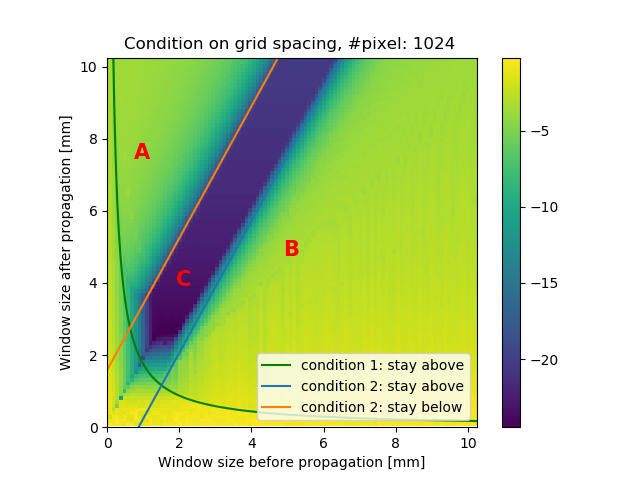
\includegraphics[width=0.45\textwidth]{npixel1024-prop_dist23-R28-Finf_con_zone.png}
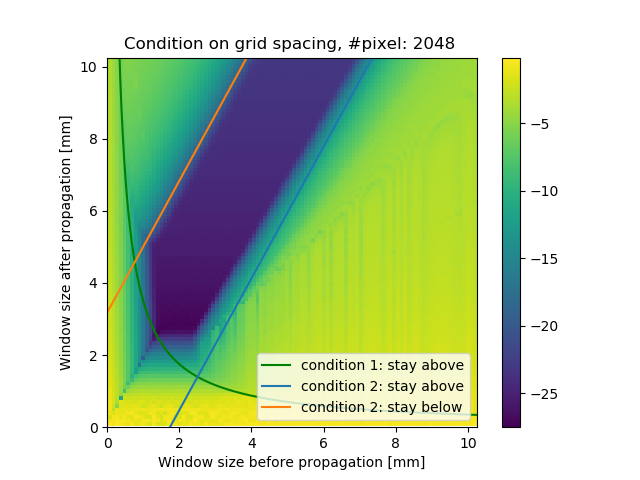
\includegraphics[width=0.45\textwidth]{npixel2048-prop_dist23-R28-Finf.png}
\end{figure}

\subsection{The zoom propagator}
\todo{RAFAEL, please...}

\section{Discussion and examples}

\todo{
Define examples to be treated by the different codes. Compare results. Vary some sampling parameters. Benchmark timing. Some ideas [to be developed]: 


\subsection{Young-type experiment}
\todo{ plane wave, two slits, like in Fig.~\ref{fig: srw two slits}. Verify numerically the Fresnel scaling theorem}

\begin{figure}
\label{fig: srw two slits}
\caption{Propagation of a plane wavefront of photon energy 10 keV at a distance $\Delta z = 10^{-1}m$) clipped by a two circular slits. The window size $w$=10$\mu$m, diameter of apertures is $w=0.25\mu m$ centered at $x=y=\pm 1 \mu m$, number of pixels: 2048$\times$2048. The results shown have been calculated with SRW. \todo{make a better graphic}
}
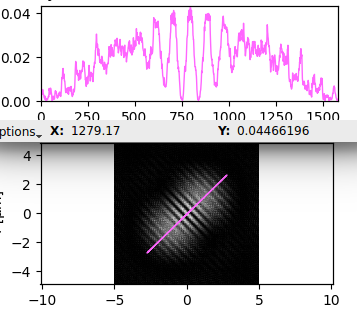
\includegraphics[width=0.95\textwidth]{srw_two_slits.png}
\end{figure}

\subsection{Approximating an undulator beam}
\todo{}
Propagate a first approximation to an undulator beam, consisting in a spherical wavefront clipped by a sort of slit with Gaussian profile.}

\subsection{Running times.}
\todo{Compare execution times of different libraries for a given example. Discuss implementations and tools.}
Figure~\ref{fig: running times 1D} compares the running times of different implementations of 1D propagators. Some conclusions can be extracted. The integral implementation with a double loop in python \{tt xwp-exact\_prop} is very slow and unmanageable, even for small arrays (we used 2048 points). When vectorizing one loop, either directly in python in {\tt wofry-integral} or using some paralelization libraries like NUMBA in {\tt xwp-exact\_prop\_numba} the calculation times are very reasonable (for 1D) and can be used systematically. The propagators using FFT are much faster (\~ 3 orders of magnitude). Their differences come from a heavier interface (in wofry, than becomes slower than xwp when accumulating 10 or more runs). Note also that {\tt fft\_conv} that uses {\tt numpy.conv} for convolution is slower than the direct implementation of two FFTs in {\tt fft}.   

\begin{figure}
\label{fig: running times 1D}
\caption{Running times in a linux/ubuntu box (Intel Xeon CPU E5-1620 3.50 GHz x 8. 16 GiB) for running the example shown in Fig.~\ref{fig: aperture_1D} with different propagators available in WOFRY (red) and XPW (blue) libraries. \ingreen{aperture\_1D\_benchmarking.py}
}
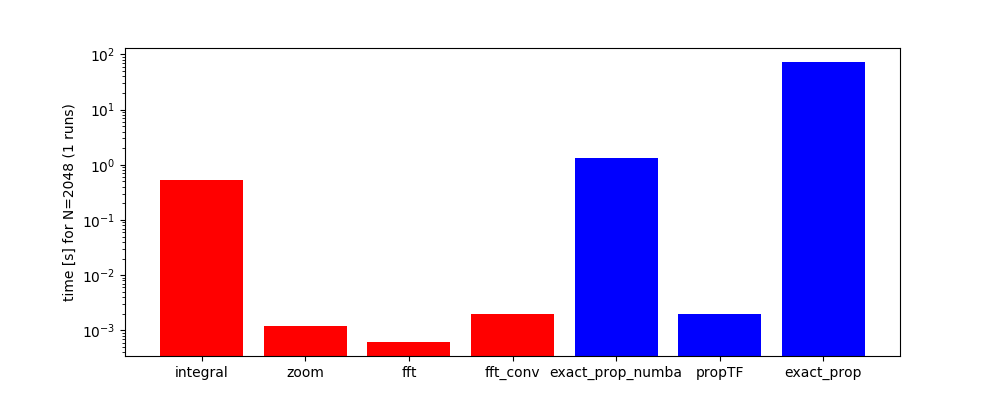
\includegraphics[width=0.95\textwidth]{aperture_1D_benchmarking.png}
\end{figure}




\section{Summary and conclusions}

\todo{Think about future directions}

%
%%%%%%%%%%%%%%%%%%%%%%%%%%%%%%%%%%%%%%%%%%%%%%%%%%%%%%%%%%%%%%%%%%%%%%%%%%%%%%%%%%%%%%%%%%%%%%%%%%%%%%%%%%%%%%%%%%%%%%%%%%%%%%%%%%%%%%%%%%%%%%%%%%%%%%%%%
%
\ack{Acknowledgements}
A large part of this work comes from ...

\appendix
\section{Fourier Transform and FFT}
\label{appendix_fft}

\todo{If the appendixes are too long, they can be moved to supplementary material.}

The Fourier Transform of a complex-valued function $g$ of two variables ($x$,$y$) is (see e.g., Ref.~\cite{goodmanfourier}): 

\begin{equation}
\tilde{g}(\tilde{x},\tilde{y}) = \int_{-\infty}^\infty \int_{-\infty}^\infty g(x,y) e^{-2 \pi i (\tilde{x}x + \tilde{y}y)} dx dy \equiv \mathcal{F}[g]
\end{equation}

and its inverse transform is: 

\begin{equation}
g(x,y) = \int_{-\infty}^\infty \int_{-\infty}^\infty \tilde{g}(\tilde{x},\tilde{y}) e^{2 \pi i (\tilde{x}x + \tilde{y}y)} d\tilde{x} d\tilde{y} \equiv \mathcal{F}^{-1}[\tilde{g}]
\end{equation}

Most programs use the Fast Fourier Transform algorithm (FFT) to compute a discrete approximation to the Fourier transform. The discrete FFT of an N-point array
$u_n$ is defined to be

\begin{equation}
 c_m = \sum_{n=0}^{N-1} u_n e^{-2 \pi i \frac{n m}{N}}
\end{equation}

for m = 0, 1, ..., N-1. The algorithm requires that N be a power of 2. For a real input function $u_n$, $c_{N-m}^\ast = cm$, which has the effect of transposing the output spectrum about $N/2$. The folding can be removed with the library operator {\tt fftshift}. Otherwise,the discrete transform is, for our purposes, equivalent to the ideal Fourier transform.

Note that different references use slightly different definitions of the Fourier transform (see, for example, \inblue{https://reference.wolfram.com/language/ref/FourierTransform.html}). The differences reside in the sign and $2 \pi$ factor of the exponent and a normalization factor. We use the definition used by Ref.~\cite{goodmanfourier} which matches well the numerical implementation of FFT in numpy. This is an important factor that must be consider in the equations and when using FFT libraries. With any representation, the Fourier transform of a Gaussian is always a Gaussian but different normalization and constant factor in the exponent may appear. With our representation:
\begin{equation}
\mathcal{F}\left\{ e^{A x^2} \right\} = \sqrt{\frac{\pi}{-A}} e^{\frac{\pi^2}{A} f_x^2}
\end{equation}
and also
\begin{equation}
\mathcal{F}^{-1}\left\{ e^{A f_x^2} \right\} = \sqrt{\frac{\pi}{-A}} e^{\frac{\pi^2}{A} x^2}
\end{equation}

\todo{One can discuss also here the particular case of FR with kernel $\exp(ik_x x)$ as used in the Section~\ref{ch: theory} because in this case the FT of a Gaussian has different coefficients as happens in Eq.~\ref{eq: Fresnel approx of angular spectrum} ??}

\section{The Fresnel Scaling Theorem}
\label{appendix_scaling}

Following Appendix B of Paganin's book \cite{paganin_book}, we consider a monochromatic scalar wave propagating from a plane at position $A$ in the negative region of a nominal optic axis $z$, to a plane in position $z=\Delta$. Suppose that the source is far enough so that the radiation can be considered paraxial, making the Fresnel approximation applicable. Consider the interaction with any element (i.e. a slit or a weakly scattering object) in position $z=0$ that generates a diffraction pattern on the plane at position $z=\Delta$. 

\vspace{0.5 cm}
\begin{figure}
\caption{Fresnel scaling theorem optical system's schematics. The schematics show the optical systems considered in the statement of the Fresnel scaling theorem. On the left a monochromatic point source, distant R from the object plane, emits X-Rays, that after passing through a slit at position $z=0$ on the optical axis ($z$), generate a diffraction pattern on a plane at position z=$\Delta$. The geometric magnification of the image $M$ is given by the relation $(R+\Delta)/R$. On the right se same system is illuminated by plane waves generating a diffraction pattern at a distance $z=\Delta/M$. The Fresnel scaling theorem states that the two diffraction patterns are identical provided that a rescaling of the complex amplitude and of the coordinates is performed.} 
\centering
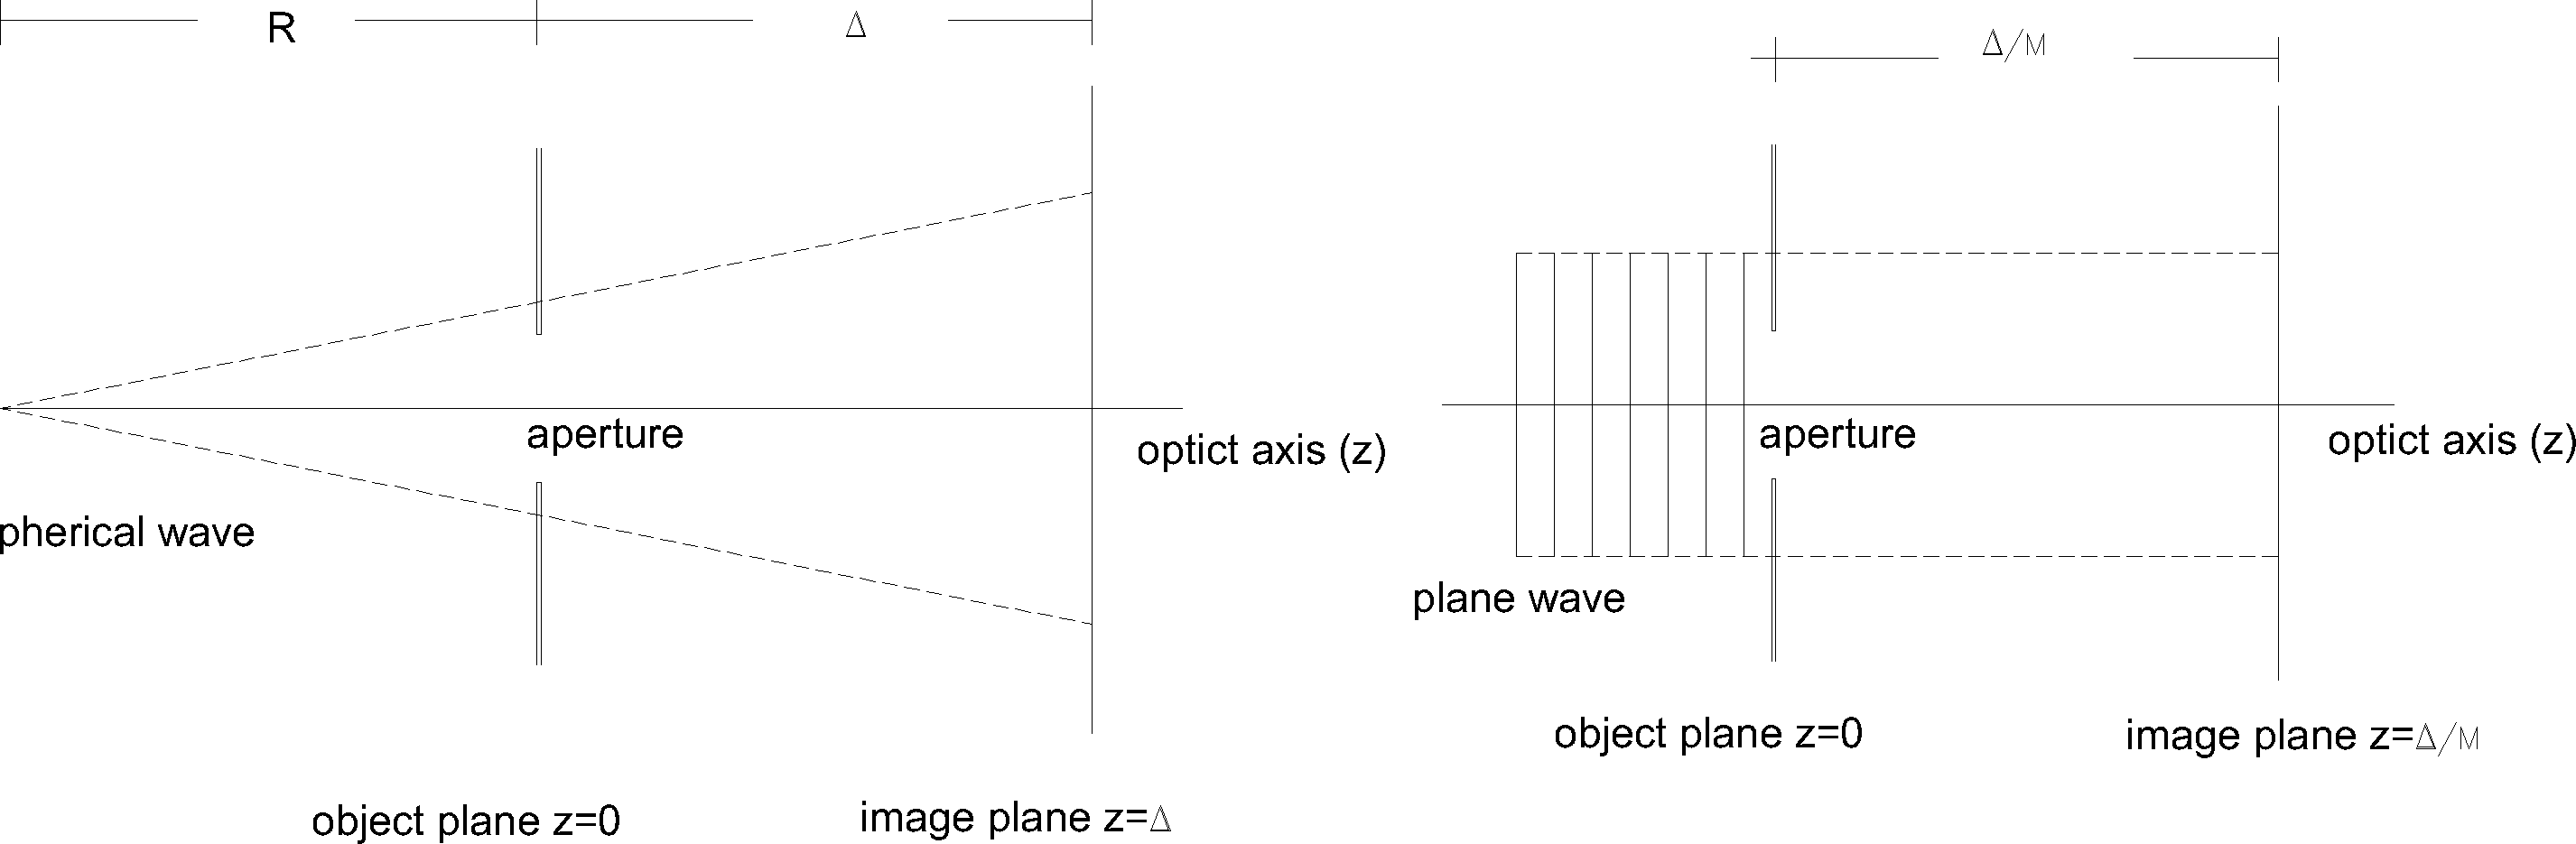
\includegraphics[width=1\textwidth]{./grafico_gio_paga.png}

\end{figure}

Given these initial conditions the theorem states that, the Fresnel diffraction pattern will have a geometric magnification $M$ which depends on the source-to-sample distance $R$, together with the sample-to-detector distance $\Delta$. If we consider the limiting case of a source at an infinite distance $R=\infty$, namely the case of a plane wave illuminating the object, we get a unit magnification. In this framework the Fresnel scaling theorem provides a simple mapping between the Fresnel diffraction pattern of an object which is obtained for the case of illumination by a point source, and a Fresnel diffraction pattern obtained for the limiting case of a plane-wave illumination. To retrieve the relation that links this two cases let's consider the plane-wave-illuminated Fresnel diffraction pattern, obtained over a plane at a propagation distance $z=\frac{\Delta}{M}$ downstream of the exit surface of the object and let's transversely magnify it by a factor $M$ and finally multiply the result buy a phase term and divide by a factor $M$. The derivation of this theorem provides an explanation of the effects of the mathematical manipulation introduced in the $2FFT$ propagator shown in the previous section (cf. equation \ref{eq: final form of Fresnel zoom in convolution form}).

Starting from equation \ref{eq: explicit form of convolution integral for propagation} and recasting it in the form:

\begin{multline}
U^{(R)}(x, y, \Delta)=\frac {e^{ik\Delta}}{ i \lambda \Delta z} e^{\big[\frac{ik}{2\Delta}(x^2+y^2)\big]} \int_{-\infty}^{\infty} \int_{-\infty}^{\infty}U^{(R)}(x^\prime, y^\prime, 0)\\ e^{ \frac{ik}{2 \Delta} [(x^\prime)^2 + (y^\prime)^2]}e^{\big[\frac{-ik}{\Delta}(xx^{\prime}+yy^{\prime})\big]} dx^\prime dy^\prime
\end{multline}

where $U^{(R)}(x, y, \Delta)$ denotes the monochromatic scalar wave-field impinging over the plane $z=\Delta$ and the $R$ superscript indicates the distance of the source from the object. Under the paraxial approximation the wavefront $U^{(\infty)}(x, y, 0)$ illuminating the object by a plane wave and $U^{(R)}(x, y, 0)$ illuminating the object by a spherical wave are related via:

\begin{equation}\label{eq: spehrical wave vs plane wave}
U^{(R)}(x, y, 0)=U^{(\infty)}(x, y, 0)e^{\big[\frac{ik}{2R}(x^2+y^2)\big]}
\end{equation}
 
Having written relation \ref{eq: spehrical wave vs plane wave} between the unpropagated wave at the plane $z=0$ for the case of the plane-wave illumination and the point-source illumination, it is possible to seek the relation between the complex-amplitude of the propagated fields:

\begin{multline}\label{eq: Fresnel rescaling not manipulated}
U^{(R)}(x, y, \Delta)=\frac {e^{ik\Delta}}{ i \lambda \Delta z} e^{\big[\frac{ik}{2\Delta}(x^2+y^2)\big]} \int_{-\infty}^{\infty} \int_{-\infty}^{\infty} U^{(\infty)}(x^\prime, y^\prime, 0)\\
e^{\big[\frac{ik}{2}(x^{\prime 2}+y^{\prime 2})\big(\frac{1}{\Delta}+\frac{1}{R}\big)\big]}e^{\big[\frac{-ik}{\Delta}(xx^{\prime}+yy^{\prime})\big]} dx^\prime dy^\prime
\end{multline}

To proceed further it necessary to specify the the form of the geometric magnification $M$:

\begin{equation}
	M= \frac{R+\Delta}{R}
\end{equation} 

so that:

\begin{equation}
	\frac{1}{\Delta}+\frac{1}{R} = \frac{1}{\Delta}\Big(\frac{R+\Delta}{R}\Big)=\frac{M}{\Delta}
\end{equation}

substituting the above expression into equation \ref{eq: Fresnel rescaling not manipulated} we arrive to:

\begin{multline}\label{eq: Fresnel rescaling with M}
U^{(R)}(x, y, \Delta)=\frac {e^{ik\Delta}}{ i \lambda \Delta} e^{\big[\frac{ik}{2\Delta}(x^2+y^2)\big]} \int_{-\infty}^{\infty} \int_{-\infty}^{\infty} U^{(\infty)}(x^\prime, y^\prime, 0)\\
e^{\big[\frac{ikM}{2\Delta}(x^{\prime 2}+y^{\prime 2})\big]}e^{\big[\frac{-ik}{\Delta}(xx^{\prime}+yy^{\prime})\big]} dx^\prime dy^\prime
\end{multline}

If we take the limit of $R\rightarrow\infty$ in the formula above, so that $M\rightarrow 1$, we see that:

\begin{multline}\label{eq: Fresnel rescaling with M=1}
U^{(\infty)}(x, y, \Delta)=\frac {e^{ik\Delta}}{ i \lambda \Delta} e^{\big[\frac{ik}{2\Delta}(x^2+y^2)\big]} \int_{-\infty}^{\infty} \int_{-\infty}^{\infty} U^{(\infty)}(x^\prime, y^\prime, 0)\\
e^{\big[\frac{ik}{2\Delta}(x^{\prime 2}+y^{\prime 2})\big]}e^{\big[\frac{-ik}{\Delta}(xx^{\prime}+yy^{\prime})\big]} dx^\prime dy^\prime
\end{multline}

In order to compare the two equations \ref{eq: Fresnel rescaling with M} and \ref{eq: Fresnel rescaling with M=1} and find the maps that link them let's make the two integrals match. First considering distance of propagation for the case of the plane wave to be $\Delta^{(\infty)}=\frac{\Delta^{(R)}}{M}$ (where the superscript in this case has been added to make clear which coordinate are taken into consideration in the two formulas) so that equation \ref{eq: Fresnel rescaling with M=1} becomes:

\begin{multline}\label{eq: Fresnel rescaling with M=1 and delta/M}
U^{(\infty)}\Big(x, y, \frac{\Delta}{M}\Big)=\frac {Me^{\frac{ik\Delta}{M}}}{ i \lambda \Delta} e^{\big[\frac{ikM}{2\Delta}(x^2+y^2)\big]} \int_{-\infty}^{\infty} \int_{-\infty}^{\infty} U^{(\infty)}(x^\prime, y^\prime, 0)\\
e^{\big[\frac{ikM}{2\Delta}(x^{\prime 2}+y^{\prime 2})\big]}e^{\big[\frac{-ikM}{\Delta}(xx^{\prime}+yy^{\prime})\big]} dx^\prime dy^\prime
\end{multline}

and then considering rescaled coordinates $(x,y)$ so that $(Mx^{(\infty)},My^{(\infty)}) = (x^{(R)},y^{(R)})$:

 \begin{multline}\label{eq: Fresnel rescaling with M=1 and delta/M and x/M}
 U^{(\infty)}\Big(\frac{x}{M}, \frac{y}{M}, \frac{\Delta}{M}\Big)=\frac {Me^{\frac{ik\Delta}{M}}}{ i \lambda \Delta} e^{\big[\frac{ik}{2\Delta M}(x^2+y^2)\big]} \int_{-\infty}^{\infty} \int_{-\infty}^{\infty} U^{(\infty)}(x^\prime, y^\prime, 0)\\
 e^{\big[\frac{ikM}{2\Delta}(x^{\prime 2}+y^{\prime 2})\big]}e^{\big[\frac{-ik}{\Delta}(xx^{\prime}+yy^{\prime})\big]} dx^\prime dy^\prime
 \end{multline}

By easily check by direct substitution of the integrals in formulas \ref{eq: Fresnel rescaling with M} and \ref{eq: Fresnel rescaling with M=1 and delta/M and x/M}:

\begin{equation}
	U^{(R)}(x, y, \Delta)= \frac{1}{M} e^{\big[ik\Delta \big({1-\frac{1}{M}}\big)\big]} e^{\big[\frac{ik}{2\Delta}(x^2+y^2)\big(\frac{M-1}{M}\big)\big]} U^{(\infty)}\Big(\frac{x}{M}, \frac{y}{M}, \frac{\Delta}{M}\Big)
\end{equation}

By rewriting equation \ref{eq: final form of Fresnel zoom in convolution form} showing a unique scaling factor $m$ for direction $x$ and $y$ and changing the variable name from $\Delta z$ to $\Delta$ we obtain:

\begin{equation}
	\begin{aligned}
	U(x_2, y_2) = &\frac { e^{ik\Delta}}{m} e^{\frac{ik}{2 \Delta} \big[(x_2^2 + y_2^2)\big(\frac{m - 1}{m}\big)\big]}\\ &\mathcal{F}^{-1}\Big[\mathcal{F}\big[U(\frac{x_2}{m}, \frac{y_2}{m})e^{\frac{ik}{2 \Delta } [(1-m)(x_1^2+y_1^2)]}\big]\times e^{-i \pi \lambda \Delta m \big(\frac{f_x+f_y}{m}\big)^2 }\Big]
	\end{aligned}
\end{equation}

The expression can be seen as the result of the Fresnel scaling theorem in the Fourier spatial-frequency domain. In fact, the Fourier transform of the unpropagated field, to which a new spherical phase term is added, is propagated to a distanced $m\Delta$ upon a rescaling of the coordinates of the spatial-frequency domain $\frac{f_x+f_y}{m}$. Taking into account a rescaling of the coordinates following the similarity theorem (cf. Eq. \ref{eq: similarity theorem}) so that a shrink in the spatial coordinated correspond to an expansion of the Fourier spatial-frequency coordinates and vice versa, the effect obtained is the propagation of the wavefront with a zooming effect.


\section{The Semianalytical treatment of the Phase}
\label{appendix_srw}
Let us suppose that our disturbance $U(x,y)$ can be factorized in a spherical-like term $U_S$ and a "flattened" residual disturbance $U_F$: 
\begin{equation}\label{eq: toroidal_phase}
	\begin{aligned}
	U(x, y) = & U_F(x,y) U_S(x,y;R_x,R_y,x_0,y_0) = \\
	          & U_F(x,y) e^{i k \frac{(x-x_0)^1}{2R_x}+i k \frac{(y-y_0)^1}{2R_y}}
\end{aligned}
\end{equation}
where $x_0$ and $R_X$ are the center and radius of a spherical wavefront matching the horizontal field curvature and similarly for the vertical with center $y_0$ and radius $R_y$. 

Introducing \ref{eq: toroidal_phase} in the Fresnel propagator one obtains the propagated field: 
\begin{equation}\label{eq: srw spherical phase}
	\begin{aligned}
	U(x, y, L) = P_G \mathcal{F}^{-1} \left\{  
	    \mathcal{F} \left\{ U_F \right\}
	    \mathcal{F} \left\{ h_S \right\}
	                                      \right\}
\end{aligned}
\end{equation}
with a global phase:
\begin{equation}\label{eq: srw global phase}
	P_G =  \frac{k}{2 \pi i L} e^{i k L + i k \frac{(x-x_0)^2}{2 R_x}+ i k \frac{(y-y_0)^2}{2 R_y}}
\end{equation}
and a kernel in real space: 
\begin{equation}\label{eq: srw global phase}
	h_S =  e^{
	  i k \frac{R_x+L}{2 R_x L} \left( x_1 - \frac{R_x x + L x_0}{R_x + L } \right) ^2 + 
	  i k \frac{R_y+L}{2 R_y L} \left( y_1 - \frac{R_y y + L y_0}{R_y + L } \right) ^2
	         }
\end{equation}

This kernel has Gaussian form $h_g = \exp{i k A x^2 + i k B y^2}$ which Fourier transform is: 
\begin{equation}
    \mathcal{F} \left\{ h_g \right\} = \frac{\pi}{\sqrt{-i k A}\sqrt{-i k A}} 
    e^{- \pi^2 i \frac{B f_x^2 + A f_y^2}{k A B}}
\end{equation}
where $A=R_x+L)/(2 R_x L))$ and $B=R_y+L)/(2 R_y L))$ and the spatial frequencies $f_x$ and $f_y$ are obtained from the transformed coordinates $x \rightarrow (r_x x + L x_0)/(R_x + L)$ and similarly $y \rightarrow (r_y y + L y_0)/(R_y + L)$

\todo{OLEG: is that correct? Please update!}


\section{The Zoom Propagator}
\label{appendix_zoom}

Expression \ref{eq: numerical convolution form of angular spectrum} provide a fast way of propagating a wavefront from the source plane to the observation plane; however it does not provide any mean of changing final window size. The sampling of the source field is conserved when using discrete Fourier transform such as $FFT$. Therefore it will fails for example resolving a small spot obtained, for example, when propagating to the waist a converging wavefront. The consequence is the need of a source oversampling which can saturate the computer memory and use a long time to perform the calculation. For this reason, a simple mathematical trick, the insertion of a magnification factor $m$ to give the possibility to modify image plane window size, and consequently the pixel size (the number of points will be conserved). The apparent effect looks like observing the propagated wavefront with a zoom. Following the approach of J. Schmidt \cite{schmidt}, the quadratic argument of the exponential that appears in equation \ref{eq: explicit form of convolution integral for propagation} is modified in order to introduce a magnification factor. However, because optical elements used at synchrotron beamlines have usually uncorrelated effects for vertical and horizontal direction, (e.g. mirrors focusing only along one direction or rectangular aperture) we modify both the $(x - x^\prime)^2$ and the $(y - y^\prime)^2$ terms to introduce two magnification factors $m_x$ and $m_y$, that act independently for the two coordinates $x$ and $y$. Here the procedure is shown only for the $x$ variable, but the same must be done for the $y$ variable as well: 

\begin{align}\label{eq:introduction of m factor}
(x_2 - x_1)^2 &= x_2^2 + x_1^2 -2 x_1 x_2 \nonumber \\
&=x_2^2 + \frac{x_2^2}{m_x} - \frac{x_2^2}{m_x} - 2 x_1 x_2 + x_1^2 + m_x x_1^2 - m_x x_1^2 \nonumber\\
&=\frac {x_2^2}{m_x} + \Big ( 1- \frac{1}{m_x}\Big) x_2^2 -2 x_2 x_1 + \Big [m_x x_1^2 + (1- m_x) x_1^2 \Big] \nonumber\\
&=m_x \Big [\Big(\frac{x_2}{m_x}\Big)^2 - 2 \Big( \frac{x_2}{m_x} \Big)x_1 + x_1^2\Big] + \Big(1-\frac{1}{m_x}\Big)x_2^2 + \Big(1-m_x\Big)x_1^2 \nonumber\\
&=m_x \Big (\frac{x_2}{m_x}-x_1\Big)^2 + \Big (\frac{m_x - 1}{m_x}\Big)x_2^2 + \Big(1-m_x\Big)x_1^2
\end{align}

A change of name for the coordinate is done  with respect to expressions appearing before equation \ref{eq:introduction of m factor} to better highlight that the final coordinate $x_2$ is a rescaled version of the initial coordinate $x_1$. Moreover, coordinate $z$ is now dropped since $(x_2,y_2)$ unequivocally identify the coordinate of the propagated field.
Substituting this expression in equation \ref{eq: explicit form of convolution integral for propagation}:

\begin{multline} \label{eq: propagation with m factor and no manupulation}
U(x_2, y_2) = \frac {e^{ik\Delta z }}{ i \lambda \Delta z} \int_{-\infty}^{\infty} \int_{-\infty}^{\infty}U(x_1, y_1) \times \\
e^{i \frac{k}{2 \Delta z} [m_x (\frac{x_2}{m_x}-x_1)^2 + (\frac{m_x - 1}{m_x})x_2^2 + (1-m_x)x_1^2]} \times \\
e^{i \frac{k}{2 \Delta z}[m_y (\frac{y_2}{m_y}-y_1)^2 + (\frac{m_y - 1}{m_y})y_2^2 + (1-m_y)y_1^2]} dx_1 dy_1
\end{multline}
and passing out of the integral the terms that do not depend on the integration variables:

\begin{multline}\label{eq: propagation with m factor and manipulation}
U(x_2, y_2) = \frac {e^{ik\Delta z }}{ i \lambda \Delta z} e^{i \frac{k}{2 \Delta z} [(\frac{m_x - 1}{m_x})x_2^2 + (\frac{m_y - 1}{m_y})y_2^2]} 
\int_{-\infty}^{\infty} \int_{-\infty}^{\infty}U(x_1, y_1) \times \\
e^{i \frac{k}{2 \Delta z} [m_x (\frac{x_2}{m_x}-x_1)^2 + (1-m_x)x_1^2]} \times \\
e^{i \frac{k}{2 \Delta z}[m_y (\frac{y_2}{m_y}-y_1)^2 + (1-m_y)y_1^2]} dx_1 dy_1
\end{multline}

By making a change of variables
\begin{equation} \label{eq: substitution of U}
U^{\prime\prime} (x_1, y_1) = U(x_1, y_1) e^{i \frac{k}{2 \Delta z} [(1-m_x)x_1^2 + (1-m_y)y_1^2]}
\end{equation}
we get:
\begin{multline}\label{eq: substitution of U in integral}
U(x_2, y_2) = \frac {e^{ik\Delta z }}{ i \lambda \Delta z} e^{i \frac{k}{2 \Delta z} [(\frac{m_x - 1}{m_x})x_2^2 + (\frac{m_y - 1}{m_y})y_2^2]} \times \\ \int_{-\infty}^{\infty} \int_{-\infty}^{\infty} U^{\prime \prime}(x_1, y_1)
e^{i \frac{k}{2 \Delta z} [m_x (\frac{x_2}{m_x}-x_1)^2]} \times \\
e^{i \frac{k}{2 \Delta z}[m_y (\frac{y_2}{m_y}-y_1)^2]} dx_1 dy_1
\end{multline}

and defining the scaled coordinates 
\begin{align} \label{scaled coordinates}
x_2^{\prime} = \frac{x_2}{m_x} ; ~~~ y_2^{\prime} = \frac{y_2}{m_y}
\end{align}
we obtain:
\begin{multline} \label{eq: substitution of scaled coordinates in integral}
U(m_x x_2^{\prime}, m_y y_2^{\prime}) = \frac { e^{ik\Delta z }}{ i \lambda \Delta z}e^{i \frac{k}{2 \Delta z} [(m_x - 1)m_x(x_2^{\prime})^2 + (m_y - 1)m_y(y_2^{\prime})^2]} \times \\
\int_{-\infty}^{\infty} \int_{-\infty}^{\infty} U^{\prime \prime}(x_1, y_1) 
e^{i \frac{k}{2 \Delta z} [m_x (x_2^{\prime}-x_1)^2]}
e^{i \frac{k}{2 \Delta z}[m_y (y_2^{\prime}-y_1)^2]} dx_1 dy_1.
\end{multline}
Therefore a convolution form is again obtained:
\begin{multline} \label{eq: convolution form of zoom propagation}
U(m_x x_2^{\prime}, m_y y_2^{\prime}) = \frac {e^{ik\Delta z }}{ i \lambda \Delta z} e^{i \frac{k}{2 \Delta z} [(m_x - 1)m_x(x_2^{\prime})^2 + (m_y - 1)m_y(y_2^{\prime})^2]}\\ \int_{-\infty}^{\infty} \int_{-\infty}^{\infty} U^{\prime \prime}(x_1, y_1) h_m((x_2^{\prime}-x_1),(y_2^{\prime}-y_1)) dx_1 dy_1
\end{multline}
where the function $h_m(x,y)$, which is now a scaled Fresnel propagator is defined as follows:
\begin{equation} \label{eq: scaled Fresnel propagator}
h_m(x_1 ,y_1) \coloneqq \frac {1}{ i \lambda \Delta z} e^{i \frac{k}{2 \Delta z} [m_x x_1^2 +m_y y_1^2]}.
\end{equation}

At this point it is desirable to find the analytical Fourier transform of $h_m$ to get a form that make it possible to apply equation \ref{eq: convolution theorem}:

\begin{equation} \label{eq: Fourier transform of Scaled propagator}
\mathcal{F}_{x,y} [h_m(x,y)] = \frac{1}{\sqrt{m_x m_y}} e^{-i \pi \lambda \Delta z (\frac{f_x^2}{m_x} +\frac{f_y^2}{m_y})}
\end{equation}
and by applying the convolution theorem:

\begin{multline}
\label{eq: final form of Fresnel zoom in convolution form}
U(x_2, y_2) = \frac { e^{ik\Delta z }}{\sqrt{m_x m_y} }e^{i \frac{k}{2 \Delta z} [\frac{m_x - 1}{m_x}x_2^2 + \frac{m_y - 1}{m_y}y_2^2]} \times \\
\mathcal{F}^{-1}\Big[\mathcal{F}\big[U(x_1, y_1)e^{i \frac{k}{2 \Delta z} [(1-m_x)x_1^2 + (1-m_y)y_1^2]}\big]
e^{-i \pi \lambda \Delta z (\frac{f_x^2}{m_x} +\frac{f_y^2}{m_y})}\Big]
\end{multline}

Equation \ref{eq: final form of Fresnel zoom in convolution form} represent the propagation of a wavefront $U(x,y)$ written in a form that is suitable to be computed again with $FFT$ numerically by simply substituting the $\mathcal{F}$ operation with the discrete one ($FFT$). Moreover, the introduction of an $m$ factor gives the possibility to act on the final spatial grid in order to zoom in and out.



\section{Fresnel propagation of a plane wave through an aperture}
\todo{this can be removed as it is just a copy of \cite{goodmanfourier}, but results have been used for some figures}
The propagated field given by the Fresnel diffraction equation \ref{eq: Fresnel approx of angular spectrum} can be solved analytically only in some particular cases. We summarize here following \cite{goodmanfourier} the results of diffraction of a plane wave by a 2D slit (square and circular), as they are used in the following sections. 

For the rectangular aperture the propagated field can be written as a function of the Fresnel integrals
\begin{equation}\label{eq: fresnel integrals}
C(x) = \int_0^x \cos(\pi t^2 / 2) dt;  ~~~~ S(x) = \int_0^x \sin(\pi t^2 / 2) dt;
\end{equation}
in the following form \cite{goodmanfourier}:
\begin{equation}\label{eq: analytical rectangular slit}
U(x, y, \Delta z)= \frac{e^{i k \Delta z}}{i} \mathcal{I}_x(x) \mathcal{I}_y(y)
\end{equation}
where the function $\mathcal{I}(t)$ is: 
\begin{align}\label{eq: analytical rectangular slit}
\mathcal{I}(t) = & \frac{1}{\sqrt 2}[ C(2 \sqrt{2 N_{F,t}} (1 - 2 t /t_{max}) + C(2 \sqrt{2 N_{F,t}} (1 + 2 t /t_{max})] +\\
		 & \frac{i}{\sqrt 2}[ S(2 \sqrt{2 N_{F,t}} (1 - 2 t /t_{max}) + S(2 \sqrt{2 N_{F,t}} (1 + 2 z /t_{max})]
\end{align}
and $N_F$ is the Fresnel number calculated for the $t$ direction: $N_{F,t} = t_{max}^2 / (\lambda \Delta z)$, $t_{max}$ is the half-aperture in the $t$ direction, $t=(x,y)$.
For the circular aperture, the propagated field is proportional to the integral:
\begin{equation}\label{eq: analytical rectangular slit}
R(z'; \Delta z) = \int_0^{N_F} \eta e^{i \pi \eta^2} J_0(2 \pi \eta r') d\eta 
\end{equation}
where $r'$ is a normalized radial coordinate $r' = \sqrt{(x^2 + y^2)/(\lambda \Delta z)}$, and $J_0$ the first-kind Bessel function of zeroth order. This integral has no analytical form but can be easily integrated numerically. 

In the case of Fraunhofer approximation, the integral $\madcad{I}_x(x)$ of \cite{goodmanfourier} can be integrated analytically and one obtains for the square aperture: 
\begin{equation}
\mathcad{I}(x) = \frac{2 x_{max}}{\sqrt{\lambda \Delta z}} e^{i \frac{\pi}{\lambda \Delta z} x^2 } sinc\left( \frac{x_{max}  \pi}{\lambda \Delta z} x \right) 
\end{equation}

\todo{Airy disk (circular+Fraunhofer)}

\section{Fresnel propagation of a spherical collapsing wave to its focal plane}
\todo{add notes by David}


     %-------------------------------------------------------------------------
     % The back matter of the paper - acknowledgements and references
     %-------------------------------------------------------------------------

     % Acknowledgements come after the appendices



     % References are at the end of the document, between \begin{references}
     % and \end{references} tags. Each reference is in a \reference entry.

% \begin{references}
% \reference{Author, A. \& Author, B. (1984). \emph{Journal} \textbf{Vol}, 
% first page--last page.}
% \end{references}
%\cite{knuth84}

%% Note added by Overleaf: If using bibtex, remove the "references" environment above, and uncomment the following lines.
%\bibliographystyle{iucr}
\referencelist{iucr}

%      %-------------------------------------------------------------------------
%      % TABLES AND FIGURES SHOULD BE INSERTED AFTER THE MAIN BODY OF THE TEXT
%      %-------------------------------------------------------------------------
% 
%      % Simple tables should use the tabular environment according to this
%      % model
% 
% \begin{table}
% \caption{Caption to table}
% \begin{tabular}{llcr}      % Alignment for each cell: l=left, c=center, r=right
%  HEADING    & FOR        & EACH       & COLUMN     \\
% \hline
%  entry      & entry      & entry      & entry      \\
%  entry      & entry      & entry      & entry      \\
%  entry      & entry      & entry      & entry      \\
% \end{tabular}
% \end{table}
% 
%      % Postscript figures can be included with multiple figure blocks
% 
% \begin{figure}
% \caption{Caption describing figure.}
% 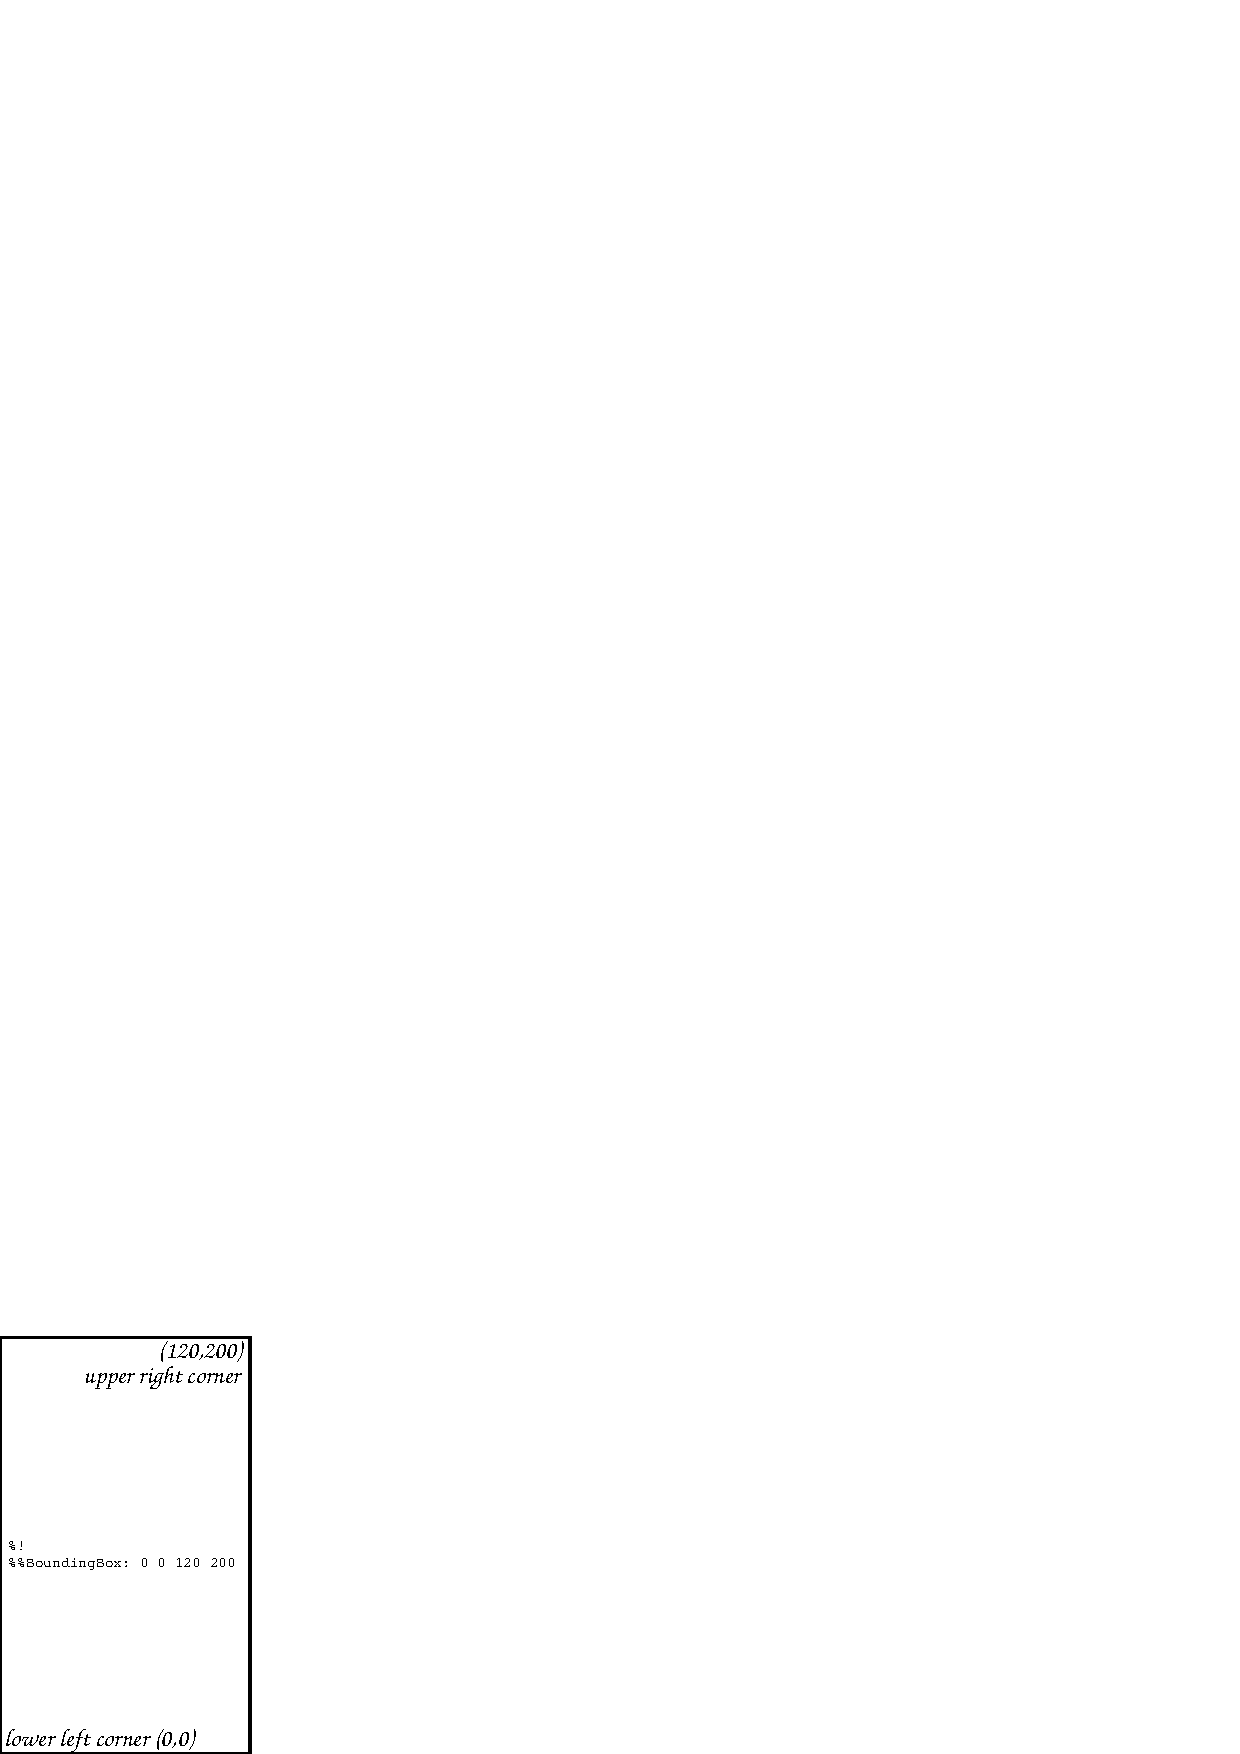
\includegraphics{fig1}
% \end{figure}


\end{document}                    % DO NOT DELETE THIS LINE
%%%%%%%%%%%%%%%%%%%%%%%%%%%%%%%%%%%%%%%%%%%%%%%%%%%%%%%%%%%%%%%%%%%%%%%%%%%%%%
